Neste capítulo, exploramos a hipótese de que a formação de câmaras de eco em uma rede social pode ser matematicamente representada através de uma combinação de várias estatísticas descritivas, cada uma correspondendo a um critério específico para a detecção de câmaras de eco. Esses critérios incluem a densidade da comunidade, a homogeneidade das opiniões, as conexões externas e o efeito de influenciadores, todos fundamentais para entender a dinâmica das redes sociais e, mais especificamente, a formação de câmaras de eco. Através da análise detalhada de cada critério e da introdução de parâmetros adicionais como o Coeficiente Individual de Câmara de Eco (ECC) e o Parâmetro Global de Câmara de Eco (GEC), buscamos desenvolver um modelo matemático que possa quantificar a probabilidade de formação de câmaras de eco em uma rede social. Este modelo é posteriormente implementado computacionalmente através da classe Python EchoChamberDetector, que utiliza algoritmos consagrados para identificação de comunidades e análise de redes sociais. A implementação permite não apenas a identificação de potenciais câmaras de eco, mas também oferece insights sobre a influência de diferentes fatores na sua formação, proporcionando uma ferramenta robusta e adaptável para análise de redes sociais no contexto da detecção de câmaras de eco.

\section{Heurísticas para detecção Câmaras de Eco}

Nossa hipótese é que a probabilidade de formação de câmaras de eco em uma rede social pode ser expressa matematicamente como uma combinação de várias estatísticas descritivas, cada uma correspondendo a um critério específico para a detecção de câmaras de eco:

\begin{itemize}
	\item \textbf{Densidade da comunidade}: A densidade da comunidade é uma medida do grau de interconexão entre os membros de uma comunidade. Em uma rede social, podemos calcular a densidade da comunidade como a proporção de conexões possíveis que realmente existem entre os membros da comunidade. Uma comunidade densa é aquela em que os membros estão altamente interconectados. Em termos de redes sociais, isso pode ser medido pelo número de conexões que cada indivíduo tem dentro de sua comunidade. Uma comunidade densa é mais propensa a formar uma câmara de eco, pois a informação circula predominantemente dentro do grupo, reforçando as opiniões existentes \cite{2015_Recuero_BOOK}.

	\item \textbf{Homogeneidade das opiniões}: A homogeneidade das opiniões refere-se ao grau de concordância ou semelhança nas opiniões dos membros de uma comunidade. Em uma rede social, isso pode ser medido pela frequência com que certas opiniões ou pontos de vista são compartilhados ou endossados pelos membros da comunidade. Quanto mais homogêneas forem as opiniões dentro de uma comunidade, maior será a probabilidade de uma câmara de eco se formar \cite{2016_WanYu}.

	\item \textbf{Conexões externas}: As conexões externas referem-se às interações entre os membros de uma comunidade e indivíduos ou grupos fora da comunidade. Em uma rede social, isso pode ser medido pelo número de conexões que cada indivíduo tem fora de sua comunidade. Quanto menor o número de conexões externas, maior a probabilidade de câmaras de eco se formarem, pois a informação é menos provável de ser desafiada por opiniões divergentes \cite{ref3}.

	\item \textbf{Efeito de influenciadores}: Os influenciadores são indivíduos ou grupos que têm um impacto significativo sobre as opiniões e comportamentos dos outros em uma rede social. Em uma rede social, isso pode ser medido pela centralidade do nó, ou seja, o número de conexões que um indivíduo tem, ou pelo número de vezes que o conteúdo de um indivíduo é compartilhado ou endossado por outros. A presença de influenciadores na rede pode influenciar a formação de câmaras de eco, pois eles podem reforçar opiniões existentes e promover a homogeneidade dentro da comunidade \cite{2014_Gilbuena}.
\end{itemize}

Antes de mergulharmos na formulação matemática, é crucial entender e definir claramente o que constitui uma "câmara de eco". Em contextos de redes sociais, uma câmara de eco é frequentemente vista como um ambiente em que os indivíduos são expostos predominantemente a informações que reforçam suas crenças e opiniões preexistentes, limitando assim a exposição a perspectivas divergentes. Este fenômeno pode resultar em polarização de opiniões e uma percepção distorcida da realidade. Além disso, ao considerar a metodologia proposta por Atiqi, é essencial destacar a relevância dos parâmetros GEC (Global Echo Chamber) e ECC (Individual Echo Chamber Coefficient). Enquanto o GEC fornece uma visão macro da tendência da rede inteira em formar câmaras de eco, o ECC se concentra na propensão individual de cada membro da rede em se isolar em tais câmaras. A inclusão desses parâmetros oferece uma abordagem mais holística, permitindo uma análise tanto no nível da rede como um todo quanto no nível individual.

No contexto da plataforma Colab, uma 'câmara de eco' pode ser definida como \textit{um subconjunto de usuários que, ao interagir predominantemente com tópicos específicos de zeladoria pública, demonstram uma homogeneidade notável em suas opiniões e perspectivas.} Esta homogeneidade é quantificada através da métrica de 'homogeneidade de opiniões', enquanto a 'average exposure' refere-se à frequência média com que um usuário é exposto a opiniões alinhadas às suas próprias opiniões dentro desses tópicos. Em essência, uma câmara de eco no Colab indica uma tendência de agrupamento de usuários que compartilham e reforçam visões semelhantes, limitando assim a diversidade de perspectivas a que são expostos.

Com base nessas hipóteses e definiçõess, podemos construir um modelo que inclua essas estatísticas descritivas. O modelo será usado para estimar os parâmetros que quantificam a influência dessas estatísticas na probabilidade de formação de câmaras de eco. Podemos expressar a probabilidade de formação de câmaras de eco como uma função de várias estatísticas descritivas:

\begin{equation}
	\begin{split}
		P(\text{{EchoChamber}}) = \exp(&\beta_1 \cdot \text{{CommunityDensity}} + \\
		&\beta_2 \cdot \text{{HomogeneityOfOpinions}} + \\
		&\beta_3 \cdot \text{{ExternalConnections}} + \\
		&\beta_4 \cdot \text{{Influencers}} + \\
		&\beta_5 \cdot \text{{AverageExposure}} + \\
		&\beta_6 \cdot \text{{GEC}} + \\
		&\beta_7 \cdot \text{{ECC}})
	\end{split}
\end{equation}

em que $\beta_1$, $\beta_2$, $\beta_3$, $\beta_4$, $\beta_5$, $\beta_6$ e $\beta_7$ são os parâmetros estimados para cada estatística descritiva e exp é a função exponencial. Essa equação fornece uma maneira de quantificar matematicamente a probabilidade de formação de câmaras de eco em uma rede social, com base nos critérios estabelecidos. Os parâmetros $\beta$ são comumente usados para quantificar a influência de várias estatísticas descritivas na probabilidade de formação de eventos complexos. Os valores dos parâmetros $\beta$ são geralmente estimados a partir dos dados. No entanto, a escolha dos valores iniciais para esses parâmetros pode ter um impacto significativo na convergência do modelo. Portanto, é comum iniciar os parâmetros beta com valores simples, como 1, e ajustá-los iterativamente para melhorar o ajuste do modelo.

Os parâmetros beta podem ser interpretados em termos de suas implicações para a probabilidade de formação de câmaras de eco. Por exemplo, um valor positivo para o parâmetro beta associado à densidade da comunidade sugeriria que comunidades mais densas têm maior probabilidade de formar câmaras de eco. Analogamente, um valor positivo para o parâmetro beta associado à homogeneidade das opiniões indicaria que comunidades com opiniões mais homogêneas têm maior probabilidade de formar câmaras de eco. Os aspectos de escala a serem considerados dependem dos critérios específicos empregados para detectar câmaras de eco. Por exemplo, ao considerar a densidade da comunidade como um critério, a escala pode ser considerada em termos do número de conexões dentro da comunidade em relação ao número total de conexões possíveis. Se a homogeneidade das opiniões for um critério, a escala pode ser considerada em termos da variação das opiniões dentro da comunidade.

\subsection{Implementação Computacional}

Para aplicar nosso teorema de probabilidade de câmaras de eco na prática, desenvolvemos a classe Python \texttt{EchoChamberDetector}. Essa classe permite analisar redes sociais e identificar potenciais câmaras de eco com base nos critérios estabelecidos em nosso teorema.

A classe \texttt{EchoChamberDetector} utiliza dois algoritmos diferentes, Louvain e também o \texttt{SignificanceVertexPartition}, uma função de classificação de comunidades disponivel no pacote \texttt{leidenalg}; para identificar comunidades dentro da rede social. Esses algoritmos são usados como etapas preliminares para identificar as comunidades da rede. Uma vez que as comunidades foram identificadas usando um dos algoritmos, prosseguimos com a análise das câmaras de eco. Para cada comunidade detectada, realizamos cálculos estabelecendo relações entre a comunidade da rede com o resto da rede como um todo:

\begin{itemize}
	\item Fator de densidade da comunidade: calculado contando a proporção de arestas existentes em relação ao número máximo possível de arestas na comunidade. Quanto maior a densidade, maior a probabilidade de formação de uma câmara de eco.
	\item Homogeneidade das opiniões: calculada a partir do desvio padrão das pontuações de opiniões dos membros da comunidade. Quanto menor o desvio padrão, maior a homogeneidade das opiniões e maior a probabilidade de formação de uma câmara de eco.
	\item Fator de conexões externas: calculado a partir da proporção de conexões da comunidade que são externas, ou seja, que se conectam a nós fora da comunidade. Quanto menor o número de conexões externas, maior a probabilidade de formação de uma câmara de eco.
	\item Fator de influenciadores: calculado a partir da proporção de de usuários com alta \textit{eigencentrality} presentes na comunidade em relação ao tamanho total da comunidade. Quanto maior a proporção de influenciadores, maior a probabilidade de formação de uma câmara de eco.
\end{itemize}

Além dessas estatísticas, também incorporamos duas heurísticas adicionais baseadas no trabalho de \citeonline{2023_Atiqi_BOOK}: Parâmetro Global de Câmara de Eco (GEC) e Exposição média.

A metodologia de cálculo do Parâmetro Global de Câmara de Eco (GEC) é baseada na abordagem apresentada por \citeonline{2023_Atiqi_BOOK}. O GEC é uma medida da tendência geral de uma rede social para formar câmaras de eco. Ele é calculado como a soma do produto dos sinais das opiniões de todos os pares de usuários conectados na rede.

Para calcular o GEC, primeiro precisamos definir a opinião de um usuário. No contexto de redes sociais, a opinião de um usuário é geralmente representada por um score que reflete a polaridade de suas postagens ou interações. Valores mais próximos de 1 representam postagens mais positivas, enquanto valores mais próximos de 0 representam sentimentos mais negativos.

Dado um par de usuários conectados $(u, v)$, o produto dos sinais de suas opiniões é dado por $\text{sign}(o_u) \cdot \text{sign}(o_v)$, onde $o_u$ e $o_v$ são as opiniões dos usuários $u$ e $v$, respectivamente, e $\text{sign}$ é a função sinal que retorna -1 para números negativos, 0 para zero e 1 para números positivos.

O GEC é então calculado somando o produto dos sinais das opiniões de todos os pares de usuários conectados na rede:

\begin{equation}
	GEC = \sum_{(u, v) \in E} \text{sign}(o_u) \cdot \text{sign}(o_v)
\end{equation}

em que $E$ é o conjunto de todas as arestas na rede.

Um valor positivo de GEC indica uma tendência para a formação de câmaras de eco, pois sugere que os usuários tendem a se conectar com outros usuários que compartilham opiniões semelhantes. Por outro lado, um valor negativo de GEC indica uma tendência para a diversidade de opiniões, pois sugere que os usuários tendem a se conectar com outros usuários que têm opiniões diferentes.

É importante notar que o GEC é uma medida global que reflete a tendência geral da rede para formar câmaras de eco. Ele não fornece informações sobre a formação de câmaras de eco em nível de comunidade ou individual. Para obter essas informações, precisamos de outras medidas ou heurísticas, como as discutidas na seção anterior.

A exposição média é outra heurística importante que Atiqi introduz em sua metodologia. Definida como a soma das diferenças entre a opinião do usuário e o sentimento da notícia exposta, média sobre todos os usuários. Matematicamente, isso pode ser expresso como:

\begin{equation}
	\text{{Exposição Média}} = \frac{1}{N} \sum_{i=1}^{N} |o_i - s_j|
\end{equation}

em que $o_i$ é a opinião do usuário $i$, $s_j$ é o sentimento da notícia $j$ exposta ao usuário $i$, e $N$ é o número total de usuários na rede.

A exposição média é uma medida de quão expostos os usuários estão a opiniões que diferem das suas. Uma alta exposição média indica que os usuários estão sendo expostos a uma variedade de opiniões, o que pode reduzir a probabilidade de formação de câmaras de eco. Por outro lado, uma baixa exposição média sugere que os usuários estão principalmente expostos a opiniões que são semelhantes às suas, aumentando a probabilidade de formação de câmaras de eco.

No contexto do Colab, a exposição média pode ser calculada aproveitando os tipos de postagens com os quais os usuários mais interagem. Cada tipo de evento, seja ele relacionado a infraestrutura, segurança pública, entre outros, pode ser representado como um número único. Isso cria um vetor de características para cada usuário que reflete os tipos de eventos com os quais ele interage. A exposição média de um usuário pode então ser calculada como a diferença entre o vetor de características do usuário e o vetor médio de características de todos os eventos na rede.

Matematicamente, isso pode ser expresso da seguinte maneira:

\begin{equation}
	\text{{Exposição Média}} = \frac{1}{N} \sum_{i=1}^{N} ||v_i - \bar{v}||
\end{equation}

em que $v_i$ é o vetor de características do usuário $i$, $\bar{v}$ é o vetor médio de características de todos os eventos na rede, e $N$ é o número total de usuários na rede. A norma $||.||$ pode ser a norma euclidiana, que mede a distância geométrica entre os dois vetores, ou outra norma apropriada.

Nesse contexto, um usuário que interage com uma variedade de tipos de eventos terá uma exposição média menor, pois seu vetor de características será mais semelhante ao vetor médio de características de todos os eventos. Por outro lado, um usuário que interage principalmente com um tipo específico de evento terá uma exposição média maior, pois seu vetor de características será mais diferente do vetor médio.

Essa abordagem permite uma análise mais granular da exposição dos usuários a diferentes tipos de eventos e pode ajudar a identificar usuários ou comunidades que estão potencialmente isolados em câmaras de eco.

\begin{itemize}
	\item \textbf{Exposição média}: A exposição média é definida como a soma das diferenças entre a opinião do usuário e o sentimento das notícias expostas, média sobre todos os usuários. Quanto maior a exposição média, maior a probabilidade de formação de uma câmara de eco, pois indica que os usuários estão sendo expostos a notícias que reforçam suas opiniões existentes.
	\item \textbf{Parâmetro Global de Câmara de Eco (GEC)}: O GEC é definido como a soma do produto dos sinais das opiniões de todos os pares de usuários conectados na rede. Um valor positivo de GEC indica uma tendência para a formação de câmaras de eco, pois sugere que os usuários tendem a se conectar com outros usuários que compartilham opiniões semelhantes.
\end{itemize}

Com base nessas estatísticas, a probabilidade de formação de câmaras de eco pode ser calculada para cada comunidade. Para representar essa probabilidade, criamos uma métrica de força de câmara de eco que é calculada como uma função exponencial das estatísticas descritivas, ponderadas pelos parâmetros beta correspondentes. Para interpretar as métricas obtidas e chegar a uma heuristica que determine quais comunidades dentro de uma rede provavelmente são câmaras de eco, realizamos uma análise para identificar os componentes principais.

\subsection{Análise de Componentes Principais}

O PCA (Principal Component Analysis) é uma técnica estatística de redução de dimensionalidade amplamente utilizada para identificar padrões em dados de alta dimensão, revelando as correlações subjacentes. No contexto das câmaras de eco, o PCA pode ajudar a desvendar quais métricas têm maior importância ou influência na determinação da presença de câmaras de eco em uma rede. Isso pode ser útil para identificar quais métricas são mais eficazes na detecção de câmaras de eco e quais métricas podem ser descartadas para simplificar o modelo. A analise revelou quatro componentes principais:

\begin{itemize}
	\item PC1 parece capturar principalmente a força da câmara de eco, a densidade da comunidade e a exposição média. Isso indica que comunidades com maior densidade e usuários com menor exposição média têm uma forte correlação com a presença de câmaras de eco.
	\item PC2 destaca a homogeneidade das opiniões e as conexões externas, porém em direções opostas. Comunidades com homogeneidade elevada e baixas conexões externas estão associadas à formação de câmaras de eco.
	\item PC3 ressalta as conexões externas e o ECC em direções opostas. Indicando que comunidades com baixas conexões externas, mas um alto ECC, podem ter propensão a ser câmaras de eco.
	\item PC4 tem forte peso na homogeneidade das opiniões e no ECC, ambos em direções opostas. Isso sugere que a presença de influenciadores e uma homogeneidade alta na opinião podem ser fatores determinantes para a formação de câmaras de eco.
\end{itemize}

\begin{figure}[htb]
	\centering
	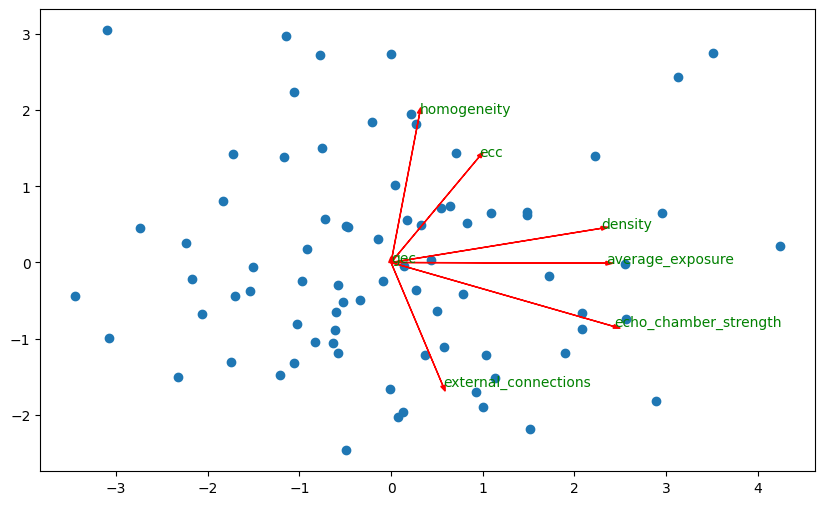
\includegraphics[width=0.7\textwidth]{images/mesquita_pca.png}
	\caption{Visualização PCA das comunidades da rede de mesquita destacando os componentes principais para formação de câmaras de eco.}
	\label{fig:mesquita_pca}
\end{figure}

Na figura \autoref{fig:mesquita_pca} podemos observar um scatterplot dos componentes ou métricas analisadas e a sua distribuição nos eixos dos dois componentes principais. O eixo x (PC1) captura a força da câmara de eco, densidade da comunidade e exposição média dos usuários. O eixo y (PC2) destaca a homogeneidade das opiniões e conexões externas em direções opostas. Cada ponto azul representa uma comunidade, evidenciando correlações entre as características mencionadas. Baseado nesses resultados, podemos propor a seguinte heurística para identificar comunidades com maior probabilidade de serem câmaras de eco:

\begin{itemize}
	\item 1. Calcular os valores para todas as métricas para cada comunidade.
	\item 2. Ponderar cada métrica pelo peso correspondente ao PCA.
	\item 3. Ordenar as comunidades com base nos valores ponderados.
\end{itemize}

Comunidades com valores altos nesta classificação terão maior probabilidade de ser câmaras de eco. Isso ocorre porque, conforme indicado pelo PCA, estas comunidades teriam alta densidade, alta força de câmara de eco e baixa exposição média, todos fatores que contribuem para a formação de câmaras de eco.

Concluindo, ao incorporar os insights do PCA com as métricas fornecidas, podemos desenvolver uma abordagem mais informada e precisa para identificar câmaras de eco em redes sociais. Esta heurística pode ser usada como uma ferramenta valiosa para moderadores e administradores de redes sociais, permitindo-lhes identificar e abordar proativamente comunidades que têm propensão a se tornarem câmaras de eco.

Essa abordagem ilustra a importância de combinar medidas globais e locais na detecção de câmaras de eco. Enquanto medidas globais como o GEC fornecem uma visão geral da tendência da rede para formar câmaras de eco, medidas locais são necessárias para identificar câmaras de eco específicas e entender a dinâmica dentro dessas comunidades. A classe \texttt{EchoChamberDetector} fornece uma implementação computacional do nosso teorema de probabilidade de câmaras de eco, permitindo a identificação de potenciais câmaras de eco em redes sociais. No entanto, é importante notar que a detecção de câmaras de eco é um problema complexo que pode não ser totalmente capturado por qualquer conjunto de heurísticas. Portanto, é sempre uma boa ideia testar essas heurísticas em uma variedade de dados e contextos para ver como elas se comportam. Nesse contexto, a análise de componentes principais nos ajudou a entender melhor quais métricas são mais importantes para a formação de câmaras de eco e como elas podem ser usadas para identificar comunidades com maior probabilidade de serem câmaras de eco.

\subsection{Derivando parâmetros beta}

Na implementação da classe EchoChamberDetector, a escolha dos valores dos parâmetros beta é um aspecto crucial para a eficácia do modelo. Esses parâmetros, que quantificam a influência de várias estatísticas descritivas na probabilidade de formação de câmaras de eco, podem ser derivados de várias maneiras, dependendo do contexto específico e das características da rede. No caso da rede social Colab, os valores dos parâmetros beta podem ser informados pelas estatísticas da rede, conforme apresentado na \autoref{tab:colab_gephi_statistics}.

O parâmetro $\beta_1$, que representa a densidade da comunidade, pode ser informado pelo coeficiente de agrupamento médio da rede. Uma rede com um coeficiente de agrupamento médio alto tende a ter comunidades densas. O parâmetro $\beta_2$, que representa a homogeneidade das opiniões, pode ser informado pelo número de comunidades na rede. Uma rede com muitas comunidades tende a ter opiniões mais homogêneas dentro de cada comunidade. O parâmetro $\beta_3$, que representa as conexões externas, pode ser informado pelo número de componentes fracamente conectados na rede. Uma rede com muitos componentes fracamente conectados tende a ter menos conexões externas. O parâmetro $\beta_4$, que representa o efeito dos influenciadores, pode ser informado pela mudança da soma da centralidade de eigenvector na rede. Uma rede com uma alta mudança da soma da centralidade de eigenvector tende a ter influenciadores mais influentes. O parâmetro $\beta_5$, que representa a exposição média, pode ser informado pelo comprimento médio do caminho na rede. Uma rede com um comprimento médio de caminho longo tende a ter uma exposição média mais alta. Finalmente, o parâmetro $\beta_6$, que representa o GEC, pode ser informado pela modularidade da rede. Uma rede com alta modularidade tende a ter um GEC mais alto.

Os valores betas derivados desse racional podem ser aplicados a rede do Colab como um todo, mas precisam ser adaptados para diferentes topologias de rede. Por exemplo o valor para numero de comunidades e o valor para numero de componentes fracamente conectados mudam drasticamente ao comprar cidades como Caruarú, Recife e Niterói, por exemplo. Dessa forma, incorporamos o cálculo desses racionais na implementação da classe \texttt{EchoChamberDetector} que calcula esses valores iniciais com base nas estatísticas da rede dado um grafo G. Isso permite uma abordagem mais informada e adaptativa para a detecção de câmaras de eco, que pode ser ajustada para diferentes redes e contextos. Para testar a classe, criamos um modelo aleatório que gera um grafo de rede social com pelo menos uma câmara de eco.

\section{Simulações de Câmaras de Eco com Modelos Aleatórios}

A análise de redes sociais é um campo que se beneficia significativamente da aplicação de modelos estatísticos, e um dos mais influentes é o modelo Markoviano. Nomeado em homenagem ao matemático russo Andrey Markov, este modelo tem sido uma ferramenta fundamental em várias disciplinas desde o início do século XX. A característica definidora de um modelo Markoviano é a sua propriedade de "sem memória", onde a probabilidade de transição para um estado futuro depende exclusivamente do estado presente, independentemente de como o sistema chegou ao seu estado atual.

Esta propriedade de "sem memória" simplifica a análise e a computação de sistemas complexos, tornando os modelos Markovianos uma escolha atraente para uma variedade de aplicações. No entanto, a aplicação dos modelos Markovianos na análise de redes sociais é particularmente interessante. Neste contexto, os nós da rede representam indivíduos ou entidades, e as arestas representam relações ou interações entre eles. Os modelos Markovianos podem ser usados para modelar a evolução dessas redes ao longo do tempo, levando em conta a dependência entre as interações.

Uma extensão desses modelos, conhecida como Modelos Exponenciais de Grafos Aleatórios (ERGMs), permite a modelagem de dependências mais complexas entre as arestas, capturando assim a estrutura de interação global da rede. Estes modelos representam uma abordagem inovadora para a análise de redes sociais, oferecendo vantagens significativas em relação aos métodos tradicionais de análise de grafos. Enquanto as técnicas tradicionais tendem a se concentrar em propriedades individuais dos nós ou arestas, os ERGMs permitem a modelagem de dependências complexas entre as arestas, capturando assim a estrutura de interação global da rede.

Os ERGMs são particularmente úteis para modelar fenômenos sociais complexos, como a formação de câmaras de eco. A análise das redes da Colab, até o presente momento, tem sido conduzida utilizando técnicas convencionais de análise de redes, tais como medidas de centralidade e modularidade, aplicadas a capturas estáticas da rede. Essas capturas representam o estado da rede em pontos específicos no tempo, fornecendo uma visão instantânea das conexões entre os usuários. O modelo de dados disponibilizado pelo Colab, apresentado em detalhes na \autoref{sec:colab_data_analysis}, consiste em uma lista de arestas que representam as conexões entre os usuários, juntamente com informações temporais que indicam quando essas conexões foram estabelecidas e possivelmente removidas. Além disso, cada usuário é caracterizado por uma série de atributos, como descrito na \autoref{tab:user_model}. A estrutura desses dados, que capturam tanto a topologia da rede quanto as características dos usuários, torna a análise baseada em ERGMs particularmente apropriada, pois permite a modelagem de dependências complexas entre as arestas, proporcionando uma representação mais precisa da estrutura de interação global da rede.

Nesse contexto, os Modelos Exponenciais de Grafos Aleatórios (ERGMs), uma extensão dos modelos Markovianos, oferecem uma abordagem metodológica robusta. Os ERGMs permitem a modelagem de dependências complexas entre as arestas, proporcionando uma representação mais precisa da estrutura de interação global da rede, mesmo em uma visão estática. Esta capacidade é particularmente relevante para a detecção de câmaras de eco, fenômenos caracterizados por comunidades altamente interconectadas dentro de uma rede, onde a informação circula predominantemente dentro do grupo. A literatura recente fornece vários exemplos de como os ERGMs podem ser usados para modelar a formação de câmaras de eco. Por exemplo, \citeonline{2022_Sun} usaram o ERGM para calcular o efeito da câmara de eco e o efeito de três mecanismos de interação na câmara de eco. Eles descobriram que o comportamento de imitação e interação entre grupos está positivamente relacionado ao efeito da câmara de eco.

\subsection{Modelando a rede social Colab com ERGMs}

O propósito de utilizar simulações ERGM neste estudo é alcançar a capacidade de criar redes sociais sintéticas que se assemelhem à rede Colab afim de testar e otimizar as heurísticas de detecção de câmaras de eco. Para atingir esse objetivo, implementamos um modelo ERGM para descrever a rede social Colab, permitindo assim a identificação e o estudo detalhado das câmaras de eco presentes nessa rede.  O modelo é especificado usando a notação formulaica do pacote ERGM, onde a fórmula define as estatísticas descritivas que descrevem a estrutura da rede e as preferências dos usuários. A seguir apresentamos a fórmula do modelo ERGM proposto para a rede social Colab:

Seja $G = (V, E)$ o grafo da rede social, onde $V$ é o conjunto de nós (usuários) e $E$ é o conjunto de arestas (conexões). Queremos modelar a probabilidade de ocorrência desse grafo com base em diferentes características e atributos dos nós e das arestas. A equação do modelo é definida como:

\[
	P(G) = \frac{e^{\sum_i \beta_i s_i(G)}}{C(\boldsymbol{\beta})}
\]

em que $P(G)$ é a probabilidade de ocorrência do grafo $G$, $\beta_i$ são os parâmetros do modelo, $s_i(G)$ são as estatísticas do modelo e $C(\boldsymbol{\beta})$ é uma constante de normalização.

As estatísticas do modelo capturam diferentes aspectos da rede social e são representadas por $s_i(G)$. Neste modelo específico, as estatísticas incluem:

\begin{itemize}
	\item $s_{\text{edges}}(G)$: O número de arestas presentes no grafo $G$. Essa estatística captura a formação de conexões entre os usuários.

	\item $s_{\text{nodematch("location")}}(G)$: O número de pares de nós que compartilham a mesma localização. Essa estatística reflete a tendência dos usuários em seguir outros usuários da mesma cidade.

	\item $s_{\text{istar(1)}}(G)$: O número de estrelas com um nó central em cada nó. Essa estatística modela a formação de conexões em torno de um usuário central.

	\item $s_{\text{ostar(1)}}(G)$: O número de estrelas com um nó central apontando para cada nó. Essa estatística captura a formação de conexões direcionadas para um usuário central.

	\item $s_{\text{nodematch("age")}}(G)$: O número de pares de nós que compartilham a mesma faixa etária. Essa estatística reflete a preferência dos usuários em seguir outros usuários da mesma idade.

	\item $s_{\text{gwidegree}}(G)$: A distribuição dos graus de entrada ponderados dos nós na rede. Essa estatística modela a propagação de popularidade entre os usuários.

	\item $s_{\text{gwodegree}}(G)$: A distribuição dos graus de saída ponderados dos nós na rede. Essa estatística captura a propagação de atividade entre os usuários.

	\item $s_{\text{nodefactor("age")}}(G)$: A distribuição dos fatores dos nós relacionados à idade. Essa estatística reflete a preferência dos usuários com base na idade.

	\item $s_{\text{gwdsp}}(G)$: A distribuição das distâncias geodésicas entre os nós na rede. Essa estatística considera a proximidade entre os usuários na formação de conexões.

	\item $s_{\text{mutual}}(G)$: O número de conexões mútuas presentes no grafo $G$. Essa estatística captura a existência de conexões bidirecionais entre os usuários.
\end{itemize}

O modelo proposto busca capturar características específicas do Colab e sua dinâmica de rede social colaborativa.

A inclusão da estatística "edges" (arestas) no modelo reflete a importância das conexões entre os usuários. No Colab, os usuários interagem uns com os outros por meio de conexões, seguindo e sendo seguidos. Essas conexões representam o fluxo de informações e colaboração na plataforma. Portanto, é essencial considerar o número de arestas presentes no grafo para modelar a formação dessas conexões.

A estatística "nodematch("location")" (correspondência de nós por localização) foi incluída para capturar a tendência dos usuários em seguir outros usuários da mesma cidade. No Colab, os usuários tendem a se conectar e colaborar com pessoas que estão geograficamente próximas a eles. Isso ocorre porque a colaboração local pode facilitar encontros pessoais, discussões presenciais e o desenvolvimento de projetos conjuntos. Portanto, ao considerar a localização como um fator de correspondência entre os nós, o modelo leva em conta essa preferência dos usuários por conexões locais.

As estatísticas "istar(1)" e "ostar(1)" foram adicionadas para modelar a formação de conexões em torno de um usuário central e a existência de conexões direcionadas para um usuário central, respectivamente. No contexto do Colab, certos usuários podem desempenhar um papel central na rede, sendo altamente conectados e influentes. Esses usuários centrais são frequentemente seguidos por outros usuários e podem ser fontes de informações, ideias e colaborações. Portanto, é relevante considerar a presença de conexões centradas em nós e conexões direcionadas para nós centrais no modelo.

A inclusão da estatística "nodematch("age")" (correspondência de nós por idade) se baseia na observação de que os usuários do Colab podem ter preferências em seguir outros usuários da mesma faixa etária. Isso pode ocorrer devido a interesses comuns, experiências compartilhadas ou abordagens semelhantes para a colaboração. Ao considerar a idade como um fator de correspondência entre os nós, o modelo leva em conta essa preferência dos usuários por conexões com pessoas da mesma faixa etária.

As estatísticas "gwidegree" e "gwodegree" foram incluídas para modelar a propagação de popularidade e atividade na rede do Colab, respectivamente. No contexto da plataforma, certos usuários podem ser mais populares e ativos do que outros. A popularidade pode ser medida pelo número de seguidores de um usuário, enquanto a atividade pode ser quantificada pelo número de pessoas que um usuário segue. Essas estatísticas capturam a disseminação da popularidade e da atividade entre os usuários, refletindo a dinâmica de influência e engajamento social no Colab.

A estatística "nodefactor("age")" foi adicionada para capturar a distribuição dos fatores relacionados à idade dos usuários. No Colab, a idade pode ser um fator importante que influencia as preferências e comportamentos dos usuários. Ao considerar os fatores relacionados à idade dos usuários como uma variável categórica, o modelo pode levar em conta possíveis diferenças nas interações e padrões de conexão com base na idade dos usuários.

Por fim, a estatística "gwdsp" (distância geodésica ponderada) foi incluída para modelar a influência do caminho geodésico na formação de conexões no Colab que representa a menor distância entre dois nós na rede. Ao considerar a distância geodésica ponderada, o modelo pode capturar o efeito da proximidade e acessibilidade na formação de conexões. Isso é relevante, pois usuários mais próximos podem estar mais propensos a interagir e colaborar uns com os outros.

Ao combinar todas essas estatísticas em um único modelo, buscamos capturar as características específicas da rede social colaborativa do Colab. Essas escolhas foram baseadas em observações e conhecimentos prévios sobre a dinâmica da plataforma, levando em consideração a importância das conexões, localização, usuários centrais, preferências relacionadas à idade, popularidade, atividade, fatores categóricos e distâncias geodésicas. O modelo visa fornecer uma representação adequada e abrangente da rede do Colab, permitindo análises mais detalhadas sobre sua estrutura e dinâmica.

\subsubsection*{Implementação de ERGMs}

Criamos um conjunto de algoritmos em R descrevevendo a implementaçao do modelo ERGM criado a partir de um sub-sampling do modelo de dados original do Colab contendo 10.000 vértices. Esse grafo original foi utilizado para simulação de grafos de rede com a intenção de converger em um grafo com estrutura similar ao grafo original. O treinamento do modelo funciona por meio de iterações. Cada iteração é uma etapa em que o modelo atualiza os parâmetros com base nos dados observados da rede e compara com as redes simuladas. O objetivo é encontrar um conjunto de parâmetros que melhor explique a estrutura da rede observada.

No início do processo, definimos a fórmula do modelo, que especifica quais características da rede estamos considerando e como elas influenciam a probabilidade dessas características ocorrerem. Durante as iterações, o modelo avalia quão bem a rede observada se ajusta às redes simuladas com base na fórmula do modelo. Ele ajusta os parâmetros para melhorar a correspondência entre a rede observada e as redes simuladas. O processo continua até que o modelo atinja a convergência, ou seja, os parâmetros alcancem um estado estável em que iterações adicionais não resultem em mudanças significativas nos valores dos parâmetros. Ao final das iterações, obtemos as estimativas finais dos parâmetros, que refletem a influência de cada termo na fórmula do modelo na probabilidade de ocorrerem determinadas características na rede. Essas estimativas nos fornecem insights sobre os processos subjacentes que moldam a estrutura da rede, como a formação de conexões entre os usuários com base na localização ou a preferência por seguir outros usuários da mesma faixa etária.

Após desenvolver o modelo baseado em ERGM, realizamos uma série de experimentos para avaliar sua adequação e desempenho. Primeiro, executamos o modelo em nossa rede social colaborativa do Colab, usando o conjunto de dados completo com 10.000 vértices. Em seguida, executamos o modelo em uma série de redes simuladas, geradas a partir do conjunto de dados original. Por fim, comparamos os resultados do modelo com os dados observados e as redes simuladas, avaliando a adequação do modelo e a qualidade de ajuste. A Figura \ref{fig:ergm_diagnostics} mostra os resultados do diagnóstico do modelo, que inclui a comparação entre os dados observados e as redes simuladas, bem como a distribuição dos parâmetros estimados. A comparação entre os dados observados e as redes simuladas mostra que o modelo se ajusta bem aos dados, pois a rede observada está dentro do intervalo de confiança de 85\% das redes simuladas. Além disso, a distribuição dos parâmetros estimados mostra que todos os parâmetros são significativos, pois seus valores estão fora do intervalo de confiança dos parâmetros simulados. Esses resultados indicam que o modelo é adequado para representar a estrutura da rede social do Colab.

\begin{figure}[!htb]
	\caption{Diagnóstico do modelo ERGM}
	\label{fig:ergm_diagnostics}
	\centering
	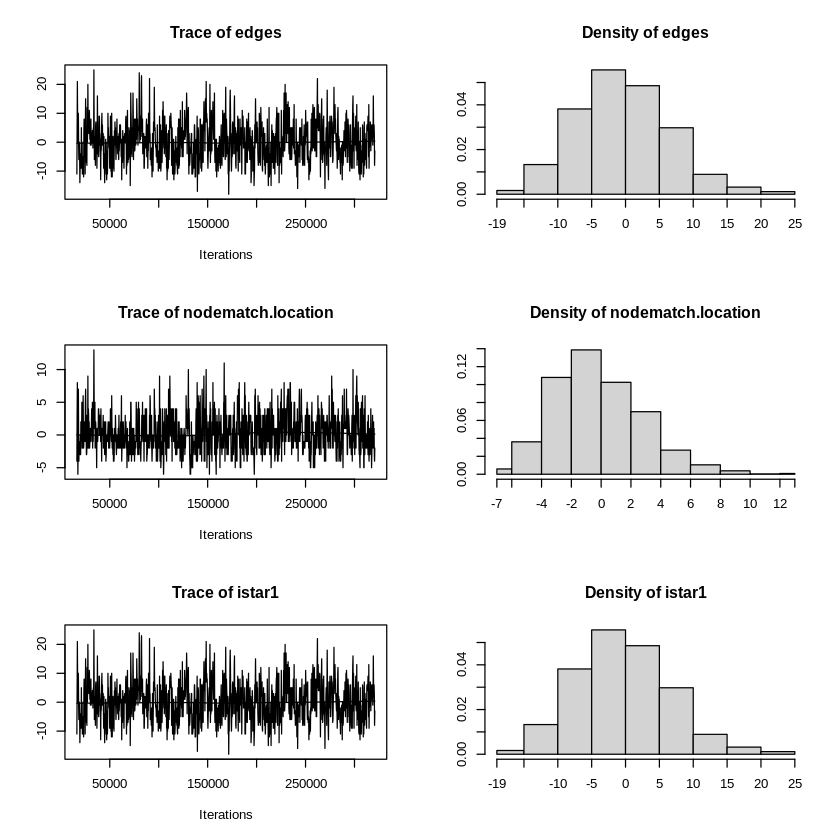
\includegraphics[scale=0.5]{images/ergm_diagnostics.png}
	\fautor
\end{figure}

Após a convergência do modelo, adotamos uma abordagem baseada em simulação para avaliar a capacidade do modelo ERGM em gerar redes que mimetizassem a estrutura da rede social do Colab. Usando o código em R, geramos vários "edgelists" de redes aleatórias. Estas redes simuladas não apenas representaram conexões entre usuários, mas também incorporaram eventos aleatórios, como curtidas e votos, indicadores de engajamento; e comentários, indicadores de diálogo; em diferentes tipos de eventos relacionados de zeladoria pública. Essa simulação foi essencial para entender o comportamento dinâmico dos usuários na plataforma. Por exemplo, é comum em redes sociais que usuários interajam mais frequentemente com postagens que são relevantes para suas próprias crenças ou interesses em sua proximidade geográfica. Ao introduzir eventos aleatórios, buscamos replicar esse comportamento com o objetivo de que as redes simuladas se assemelhassem, tanto quanto possível, à rede real do Colab.

\subsection{Visualizando Câmaras de Eco em redes simuladas}

De volta ao Python, podemos utilizar a classe \texttt{NetworkPlotter} para exibir a rede com os nós colorizados baseado nas comunidades identificadas. A \autoref{fig:ergm_random_network} ilustra o plot de uma das redes geradas. Ao observar a imagem da rede simulada, é possível identificar diversas características que podem ser correlacionadas com o comportamento observado nas redes do Colab:

\begin{itemize}
	\item \textbf{Clusters Distintos:} A presença de grupos coloridos distintos na visualização sugere a formação de comunidades. Alguma das comunidades podem ser consideradas câmaras de eco, especialmente quando indivíduos com interesses ou opiniões semelhantes tendem a interagir mais entre si do que com outros membros da rede.
	\item \textbf{Conexões Inter-Comunidades:} Ainda que existam clusters distintos, é notável que há diversas conexões entre eles. Isto pode indicar a presença de usuários "ponte", que interagem com múltiplas comunidades e podem ser essenciais na difusão de informações entre grupos diferentes.
	\item \textbf{Densidade Variável:} Algumas comunidades parecem ser mais densamente conectadas do que outras. Isto pode ser um indicativo de grupos mais ativos ou com maior engajamento na plataforma. No contexto do Colab, isso poderia representar comunidades mais engajadas em discussões ou atividades de zeladoria pública.
	\item \textbf{Centralidade Variável}: A \textit{eigencentrality}, representada pelo tamanho dos nós, indica que existem alguns usuários que são mais centrais do que outros. Isto pode ser um indicativo de usuários com maior influência na rede, que podem ser considerados líderes de opinião ou influenciadores.
\end{itemize}

\begin{figure}[!htb]
	\caption{Plot de um rede aleatória gerada pelo modelo ERGM baseado na topologia da rede do Colab}
	\label{fig:ergm_random_network}
	\centering
	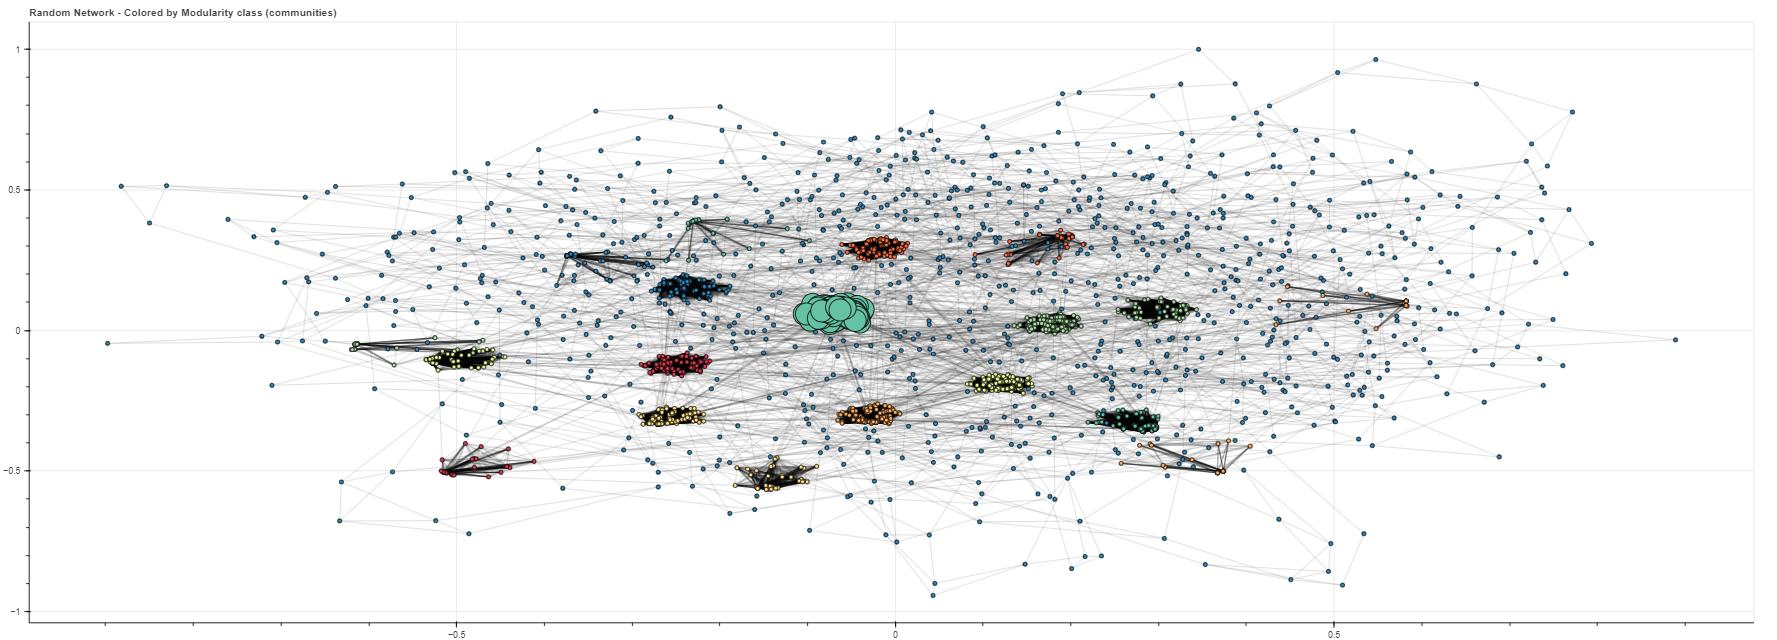
\includegraphics[width=0.9\textwidth]{images/ergm_random_network.png}
	\fautor
\end{figure}

\begin{figure}[!htb]
	\caption{Plot da topologia da rede de usuários Colab no Rio de Janeiro}
	\label{fig:network_plot_rio_de_janeiro}
	\centering
	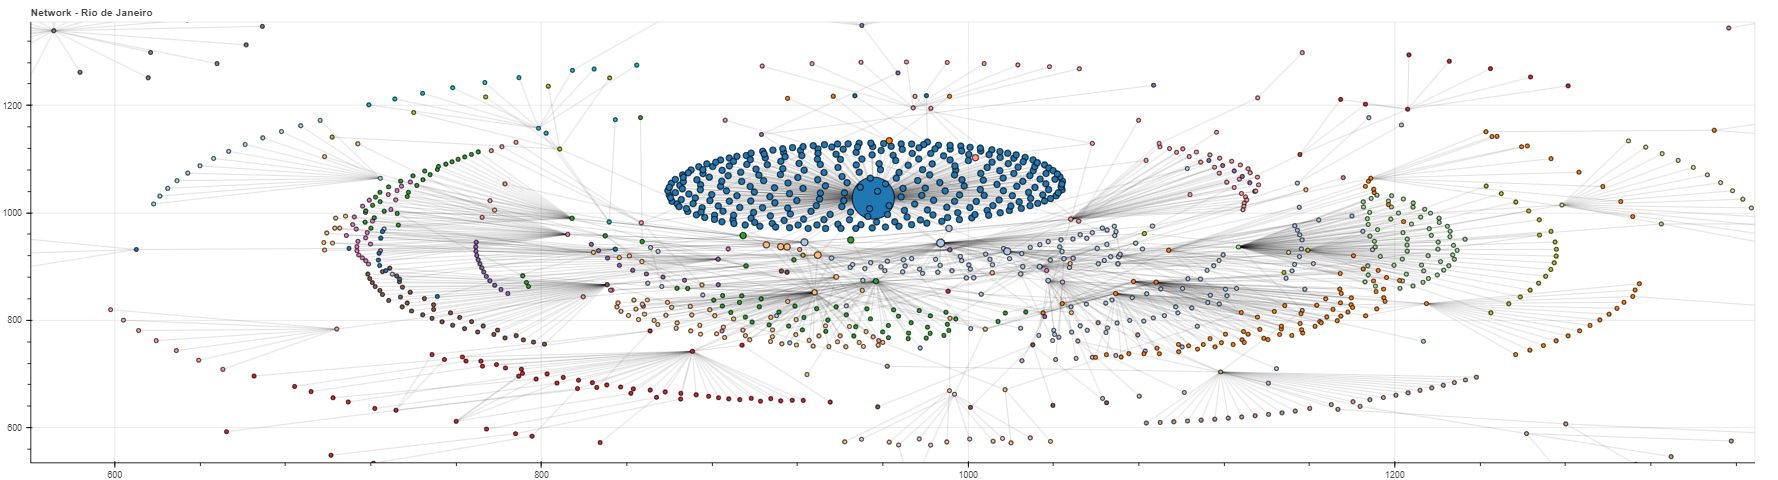
\includegraphics[width=0.9\textwidth]{images/network_plot_rio_de_janeiro.png}
	\fautor
\end{figure}

Estas observações reforçam a importância de considerar não apenas as conexões diretas entre os usuários, mas também suas interações com conteúdos e eventos. Para plataformas como o Colab, entender estas dinâmicas pode ser crucial para promover maior engajamento, identificar líderes de opinião ou detectar áreas de interesse emergente. Para uma validação mais empírica do modelo ERGM, podemos comparar a topologia da rede simulada com a topologia da rede real. A \autoref{fig:network_plot_rio_de_janeiro} ilustra a topologia da rede do Colab no Rio de Janeiro, enquanto a \autoref{fig:ergm_random_network} ilustra a topologia de uma rede simulada. Ao comparar as duas imagens, é possível observar que a rede simulada apresenta algumas características semelhantes à rede real:

\begin{itemize}
	\item \textbf{Concentração de Interações:} Em ambas as imagens, pode-se observar que há uma concentração significativa de nós (usuários) no centro da rede, cercados por conexões densas. Isso sugere que há usuários ou postagens específicas que são particularmente populares ou influentes na plataforma, atraindo uma quantidade desproporcional de interações. Estes poderiam ser chamados de "hubs" ou influenciadores dentro da rede.
	\item \textbf{Comunidades:} Em ambas as imagens também se observa um padrão semelhante na distribuição da comunidade, tanto em sua densidade, número de nós e nos aspectos de centralidade, destacando poucos usuários com grande influência na rede.
	\item \textbf{Hubs vs. Periferia:} Enquanto há uma densa concentração de interações no centro, a periferia da rede apresenta nós menos conectados. Estes nós periféricos podem representar novos usuários, usuários menos ativos ou postagens menos populares.
\end{itemize}

A rede simulada baseada no modelo ERGM parece replicar com sucesso muitas das características observadas na rede real do Colab. A capacidade de simular redes sociais, especialmente aquelas com características complexas e interações multifacetadas, é fundamental para avançar na pesquisa e análise de redes. A rede simulada, com base no modelo ERGM, ilustra a potência desta abordagem, ao conseguir reproduzir muitas das características intrínsecas observadas na rede real do Colab. Esta correspondência não é apenas uma validação da precisão do modelo ERGM, mas também destaca sua relevância prática na modelagem de redes sociais.

O emprego de simulações, como aquelas produzidas pelo modelo ERGM, oferece vários benefícios para os analistas de dados. Primeiramente, permite testar e validar heurísticas em ambientes controlados, reduzindo os riscos associados ao trabalho com dados reais, que podem ser ruidosos, incompletos ou distorcidos. Além disso, ao trabalhar com simulações, os analistas podem se distanciar de potenciais vieses inerentes aos dados reais, garantindo uma análise mais objetiva e imparcial. Este distanciamento das simulações dos dados reais é particularmente importante em contextos onde as interações e os padrões de comportamento dos usuários podem ser sensíveis ou privados. Ao utilizar redes simuladas, os pesquisadores podem conduzir experimentos e análises sem comprometer a privacidade ou a integridade dos usuários reais da aplicação.

A capacidade de simular redes que se assemelham às reais destaca a importante sinergia entre engenharia de software e análise de dados. Ao criar pipelines que facilitam a validação de heurísticas sociais complexas, a engenharia de software desempenha um papel crucial em potencializar a análise em contextos de democracia digital. Essas simulações proporcionam aos analistas de dados uma ferramenta robusta para coletar métricas relevantes a partir de redes simuladas, como a detecção de câmaras de eco, sem se envolver diretamente com dados reais. Isso, por sua vez, aprimora a confiabilidade das análises e otimiza os processos de tomada de decisão baseados em dados.

A utilização do modelo ERGM é um exemplo desta interseção entre engenharia, simulação e análise. A eficácia em replicar características observadas em redes reais, como a do Colab, enfatiza a importância de ferramentas e técnicas multidisciplinares para enriquecer e refinar a pesquisa e prática em análise de redes sociais.

A partir das redes simuladas, realizamos uma série de intervenções controladas para emular as características de câmaras de eco observadas em cenários reais. Inicialmente, identificamos empiricamente, avaliando as métricas de densidade, centralidade e conexões externas, comunidades dentro da simulação que apresentavam maior predisposição a se tornarem câmaras de eco, com base em atributos estruturais e dinâmicas de interação. Em seguida, manipulamos de forma direcionada os parâmetros de centralidade, densidade, conexões externas e homogeneidade de opiniões dessas comunidades, com o objetivo de fortalecer artificialmente as características inerentes às câmaras de eco.

O propósito destas manipulações foi duplo. Primeiro, queríamos assegurar que todas as redes simuladas contivessem pelo menos uma representação clara de câmara de eco, servindo como um padrão de referência. Segundo, essa configuração controlada proporcionou um cenário ideal para avaliar a eficácia do nosso algoritmo de detecção. Com a presença de uma "câmara de eco artificial" claramente definida, poderíamos quantificar o sucesso do modelo em identificar tal estrutura dentro da rede.

A eficácia do modelo de detecção foi, portanto, avaliada com base em sua capacidade de identificar e classificar corretamente estas comunidades modificadas como câmaras de eco. A abordagem empregada assemelha-se à metodologia usada em treinamentos de modelos de classificação de aprendizado de máquina, onde a presença de um padrão conhecido é fundamental para avaliar a precisão do algoritmo. Por meio deste procedimento, buscamos não apenas validar nosso modelo de detecção, mas também estabelecer um protocolo replicável para futuras investigações no campo da detecção de câmaras de eco em redes sociais simuladas.

Das dez redes simuladas examinadas, o modelo demonstrou competência ao identificar, consistentemente, a câmara de eco artificial em todas as instâncias analisadas. Nota-se, além disso, que os parâmetros GEC, ECC, densidade, homogeneidade de opiniões e centralidade para as demais câmaras de eco identificadas se alinham adequadamente com os resultados antecipados em nossa proposição inicial.

Interessantemente, uma em carácter experimental, ao alterar o algoritmo de detecção de comunidades precedente à identificação de câmaras de eco, os resultados obtidos para as comunidades identificadas apresentam variações consideráveis. Quando adotado o algoritmo padrão, que utiliza uma função de qualidade ancorada em significância para determinar as partições das comunidades, os resultados tendem a ser mais consistentes, o que faz sentido considerando a natureza direcionada do grafo da rede.

No entanto, ao empregar o algoritmo de Louvain, que possui uma propensão a consolidar comunidades menores em agrupamentos maiores, usuários pertencentes as câmaras de eco artificialmente inseridos foram alocados em comunidades diferentes da sua comunidade original, de forma que, as métricas associadas às câmaras de eco para os usuários manipulados elevaram-se a tal ponto que o sistema identificou comunidades com dimensões até o dobro das originais como alta probabilidade de serem câmaras de eco.

Curiosamente, esse fenômeno amplificado parece estar correlacionado à centralidade dos usuários nas respectivas comunidades. Tal observação sugere que a centralidade pode desempenhar um papel crítico na forma como as câmaras de eco são percebidas e detectadas. Por outro lado, ao adotar o algoritmo de Girvan-Newman, que se caracteriza por sua capacidade de identificar comunidades sobrepostas e, no entanto, demanda um tempo computacional substancialmente mais extenso, observou-se uma granularidade reduzida nas comunidades. Contudo, devido à otimização do algoritmo para identificar essas sobreposições, a comunidade associada à câmara de eco original foi replicada e corretamente identificada pelo modelo de detecção.

Essas descobertas destacam a importância da escolha do algoritmo na detecção precisa de câmaras de eco em contextos simulados, portanto, torna-se imperativo ressaltar que o algoritmo de detecção foi essencialmente considerado "calibrado" para funcionar de forma otimizada em situações em que o grafo é direcionado e as comunidades são identificadas pelo algoritmo \texttt{SignificanceVertexPartition}. O algoritmo é singular por sua capacidade de quantificar a significância estatística das partições, proporcionando assim uma compreensão detalhada e robusta sobre a estrutura intrínseca das comunidades. Essa técnica avalia a qualidade das partições, comparando a densidade de arestas dentro das comunidades com aquela esperada sob um modelo nulo.

Não obstante, cabe ressaltar que a escolha pelo algoritmo de significância não foi predeterminada na concepção original do modelo, mas sim foi fruto de um processo experimental. Ao longo da pesquisa, vários algoritmos de detecção de comunidades foram avaliados, e o de significância emergiu como o mais apropriado, especialmente devido à sua conveniência e eficácia para grafos direcionados. Anteriormente, enfatizamos que muitos algoritmos de detecção de comunidades não são intrinsecamente otimizados para lidar com grafos direcionados, uma característica que pode comprometer a acurácia da detecção de câmaras de eco.

As simulações, portanto, revelaram que, enquanto o modelo de detecção de câmaras de eco consegue consistentemente identificar a câmara de eco artificialmente inserida quando empregando o algoritmo de significância de partição de comunidades, essa consistência pode variar consideravelmente com a adoção de outros algoritmos de detecção de comunidades. A íntima relação entre as heurísticas de detecção de comunidades e detecção de câmaras de eco não é surpreendente, visto que muitas das métricas empregadas para identificar câmaras de eco derivam de metodologias clássicas de detecção de comunidades.

Dessa forma, concluímos que, ao abordar a complexa tarefa de detecção de câmaras de eco, é indispensável ponderar sobre os aspectos topológicos da rede em análise. Escolher um algoritmo de partição de comunidades alinhado com essas características topológicas pode não apenas potencializar a precisão da detecção, mas também fornecer insights mais profundos sobre as dinâmicas subjacentes das redes sociais em estudo.

\begin{figure}[!htb]
	\caption{Plot da rede ERGM com câmaras de eco identificadas}
	\label{fig:ergm_random_network_echo_chambers}
	\centering
	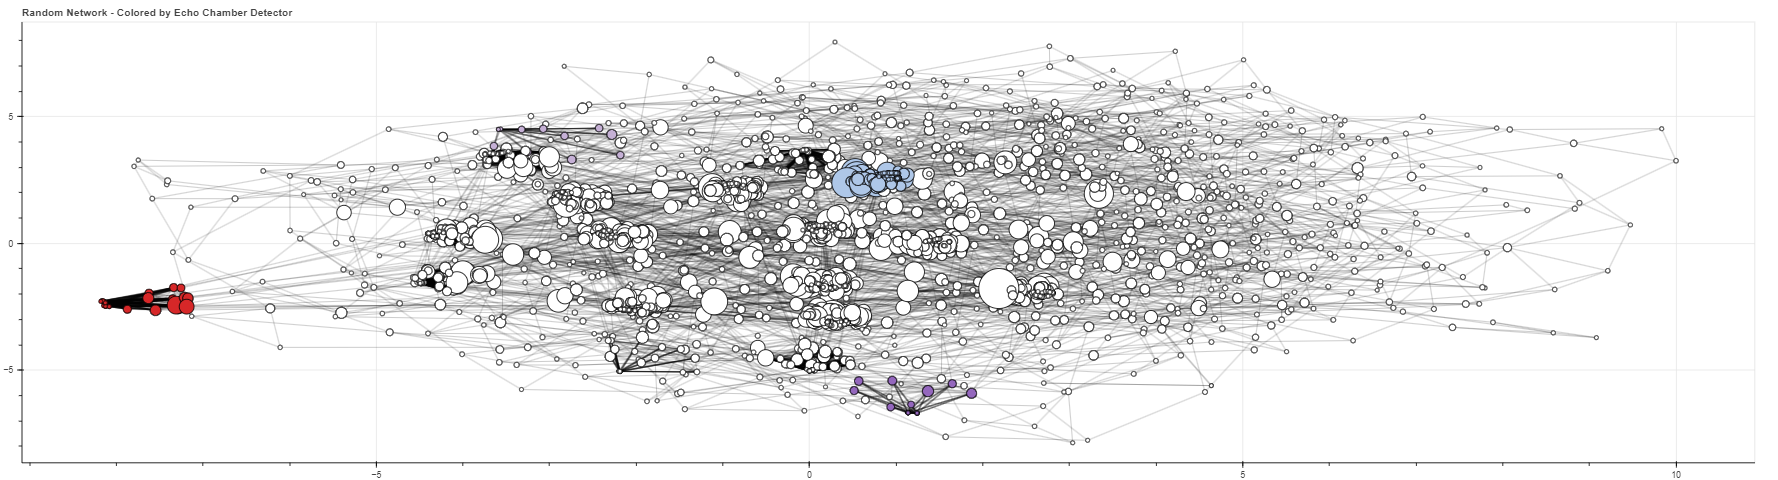
\includegraphics[width=0.9\textwidth]{images/ergm_random_network_echo_chambers.png}
	\fautor
\end{figure}

Para visualizar as câmaras de eco identificadas, criamos a visualização com diferenciação cromática clara, onde cada cor distinta representa uma câmara de eco específica e os nós em branco correspondem a atores ou entidades fora dessas câmaras. Esta representação gráfica foi concebida para permitir uma rápida identificação e análise das estruturas subjacentes destas câmaras de eco, realçando as suas relações, centralidade e densidade dentro da rede global. Na simulação da rede representada pela \autoref{fig:ergm_random_network_echo_chambers}, podemos identificar três câmaras de eco distintas, representadas pelas cores vermelha, azul e lilás.

Ao focarmos no grupo vermelho, observamos que esta câmara de eco, sendo artificialmente inserida, situa-se isolada dos demais grupos, indicando uma certa polarização e falta de interconexão com outros atores da rede. O seu posicionamento, juntamente com a proximidade entre os nós, sugere uma alta densidade interna, denotando uma possível homogeneidade de opiniões ou interações frequentes entre os membros.

Em contraste, a câmara de eco azul exibe uma estrutura mais dispersa e um posicionamento mais central na rede, o que pode indicar uma influência ou conexão mais ampla com outros atores, mesmo aqueles fora de sua câmara. Além disso, a variação no tamanho dos nós dentro dessa comunidade sugere uma hierarquia ou diferenças na centralidade de eigenvector entre os seus membros.

A câmara de eco lilás, embora menor em comparação com a azul, possui uma distribuição interessante, estendendo-se em uma direção específica e contendo nós com centralidades variadas. Isso pode indicar uma subcomunidade em formação ou um grupo com opiniões mais diversificadas.

Em geral, enquanto a câmara de eco artificial vermelha apresenta um isolamento claro, as câmaras de eco identificadas pelo modelo mostram-se mais integradas à rede. Esta visualização destaca a complexidade e a interconexão das câmaras de eco no cenário digital, enfatizando a necessidade de abordagens analíticas refinadas para compreender plenamente as dinâmicas e implicações dessas estruturas em redes sociais.

A implementação dos modelos ERGM permitiu gerar redes aleatórias que espelham com um certo grau de aleatoriedade, a rede de usuários do aplicativo Colab. Esta abordagem demonstrou ser fundamental, pois através dessas simulações foi possível validar com precisão e amadurecer o modelo de detecção de câmaras de eco previamente construído. A confiabilidade desse método se reflete na sua capacidade de discernir quais comunidades no Colab são potencialmente câmaras de eco, oferecendo assim uma ferramenta valiosa para aqueles que desejam investigar essas estruturas.

A adição do modelo de visualização, por sua vez, amplia o alcance desse método. Essa representação gráfica, interpretável empiricamente, não só beneficia os stakeholders do aplicativo Colab, como também serve como uma ferramenta instrutiva para agentes governamentais e analistas que buscam compreender a dinâmica dessas redes.

Contudo, é crucial entender a natureza quantitativa e orientativa do modelo. Enquanto ele pode indicar comunidades mais polarizadas com valores que desviam muito do padrão do grafo da rede como um todo, o modelo não rotula definitivamente uma comunidade como sendo uma câmara de eco. É uma ferramenta para guiar a análise, e não para definir conclusões. A justificativa principal para esse racional remete ao experimento de trocar o método de partição de comunidades. Quando o modelo Girvan-Newman foi usado, usuários foram incluidos em comunidades que não foram identificadas como câmaras de eco pelo modelo de significância de partição de comunidades. Isso sugere que o modelo de detecção de câmaras de eco é sensível ao método de partição de comunidades, e que a escolha de um método de partição de comunidades deve ser feita com cuidado. Por tanto, considerando essas incertezas, entendemos que a decisão final sobre a natureza de uma comunidade deve ser feita por um analista humano, que pode levar em consideração outros fatores, como a natureza dos comentários e a atividade dos usuários.

Ao realizar essas anlálises mais definitivas, por mais elucidativa que seja a perspectiva visual, é essencial reconhecer suas limitações. A representação gráfica, embora intuitiva, não projeta todas as métricas derivadas durante a análise das comunidades e da detecção de câmaras de eco. A análise dos aspectos de centralidade, densidade, conexões externas, ECC e GEC, quando comparada entre todas as comundiades da rede, pode oferecer insights muitas vezes sutis e profundamente informativos, portanto são indispensáveis para um entendimento mais robusto das origens e comportamentos das câmaras de eco em redes sociais. No próximo tópico, aprofundaremos a análise dessas métricas, dando destaque à sua relevância na compreensão das câmaras de eco nas redes de Niterói, Santo André e Mesquita.

\section{Estudo de caso das redes de Niterói, Santo André e Mesquita}

A complexidade e a dinâmica das redes sociais tornam essencial a utilização de ferramentas analíticas e representações gráficas para entender suas estruturas e comportamentos. As câmaras de eco, como fenômeno emergente nesses ambientes, desafiam os analistas a encontrar maneiras eficazes de identificá-las e compreendê-las. No entanto, a mera visualização dessas estruturas, embora poderosa, não é suficiente para capturar a totalidade do fenômeno. Como veremos nesta seção, uma investigação mais aprofundada das métricas específicas, como centralidade, densidade, conexões externas, ECC e GEC, proporciona uma compreensão mais rica e nuanceada das câmaras de eco e sua manifestação em redes específicas. Neste estudo de caso, direcionamos nossa atenção para as redes de Niterói, Santo André e Mesquita, explorando as particularidades e insights revelados por essas métricas.

\begin{itemize}
	\item \textbf{Carregamento das Redes:} As redes das respectivas cidades, previamente isoladas no Gephi, foram carregadas no formato de dataframe edgelist, sendo posteriormente convertidas em grafos direcionados utilizando a biblioteca NetworkX.
	\item \textbf{Filtragem de Dados:} Conjuntos de dados contendo postagens sobre eventos de zeladoria pública, juntamente com seus respectivos comentários, likes e votações (positivas e negativas) foram incorporados. Uma filtragem subsequente assegurou que cada cidade possuísse eventos e interações pertinentes somente aos usuários de sua rede.
	\item \textbf{Particionamento de Comunidades:} Adotou-se o modelo SignificanceVertexPartition para discernir e segmentar as comunidades de cada cidade. Através deste processo, foi possível determinar o número de comunidades, bem como os tamanhos máximo, mínimo e médio dessas comunidades.
	\item \textbf{Derivação de Parâmetros:} Com base nas características topológicas do grafo, foram derivados os parâmetros beta, essenciais para a etapa subsequente de identificação.
	\item \textbf{Detecção de Câmaras de Eco:} Através do modelo de detecção, foram identificadas comunidades com elevada probabilidade de serem câmaras de eco. Este julgamento baseou-se em métricas de análise de rede, polaridade das postagens, uniformidade dos tipos de eventos, engajamento representado por likes e votações, bem como interações como comentários e postagens.
	\item \textbf{Visualização:} Por fim, as comunidades diagnosticadas como potenciais câmaras de eco foram destacadas no gráfico. Este destaque foi baseado tanto em coloração diferenciada quanto no dimensionamento dos nós, considerando fatores de centralidade.
\end{itemize}

\subsection{Santo André}

\begin{table}[ht]
	\centering
	\caption{Métricas de Detecção de Câmaras de Eco da Rede da Cidade de Santo André}
	\label{tab:echo-chamber-metrics-santo-andre}
	\begin{tabular}{l|l}
		\toprule
		\textbf{Topologia da Rede}          & \textbf{Valor}                   \\
		\midrule
		Nós                                 & 2102                             \\
		Arestas                             & 6430                             \\
		Nº de comunidades                   & 243                              \\
		\toprule
		\textbf{Conteúdo}                   & \textbf{Valor}                   \\
		\midrule
		Tamanho da maior comunidade         & 44                               \\
		Tamanho da menor comunidade         & 3                                \\
		Tamanho médio das comunidades       & 6.56                             \\
		Nº de comentários                   & 49912                            \\
		Nº de likes                         & 165563                           \\
		Nº de votos                         & 11222                            \\
		Modularidade do grafo               & 0.5438                           \\
		\midrule
		\textbf{Polarização e Homofilia}    &                                  \\
		\midrule
		Coeficiente Global de Câmara de Eco & 0.04619                          \\
		Força da Câmara de Eco no Grafo     & 1.0743                           \\
		Nº de Câmaras de Eco Detectadas     & 4                                \\
		\midrule
		\textbf{Comunidade}                 & \textbf{Índice de Câmara de Eco} \\
		\midrule
		Comunidade 233                      & 2.0471                           \\
		Comunidade 225                      & 2.0119                           \\
		Comunidade 160                      & 1.9558                           \\
		Comunidade 207                      & 1.9112                           \\
		\bottomrule
	\end{tabular}
\end{table}

A topologia da rede de Santo André, constituída por 2.102 nós e 6.430 arestas, e a existência de 243 comunidades distintas, refletem uma topologia que favorece tanto a interconectividade quanto a fragmentação. A modularidade da rede, uma medida de quão bem a rede se divide em módulos ou comunidades, é razoavelmente alta. Isso pode indicar uma tendência para grupos isolados de discussão, onde as opiniões podem circular sem serem contestadas por visões externas, facilitando a formação de câmaras de eco.

As métricas de conteúdo, incluindo um total de 49.912 comentários, 165.563 curtidas e 11.222 votos, destacam um nível significativo de engajamento dos usuários na plataforma. A relação entre curtidas e comentários pode indicar a predisposição dos usuários a expressar concordância passiva (por curtidas) em vez de envolvimento ativo (por comentários), um comportamento que pode contribuir para a manutenção de câmaras de eco, onde a concordância é frequentemente mais visível do que o debate ou a discordância.

Para aprofundar a discussão, analisaremos cada métrica individualmente, discutindo suas implicações e como elas interagem com as outras métricas para formar um quadro mais amplo do ambiente social na plataforma. Examinaremos as nuances das interações sociais dentro das comunidades, como estas são influenciadas por fatores como a densidade e a homogeneidade, e como a limitação de conexões externas pode contribuir para a formação de câmaras de eco. Também discutiremos a presença e o papel dos influenciadores na rede e como a exposição média a opiniões alinhadas pode afetar a dinâmica da comunidade. Finalmente, integraremos estas análises com uma avaliação do coeficiente de câmara de eco global e individual, fornecendo uma visão holística da rede e suas tendências para a formação de câmaras de eco.

O Coeficiente Global de Câmara de Eco (GEC) e a Força de Câmara de Eco do Grafo (Graph Echo Chamber Strength) são indicadores críticos de quão pronunciadas são as câmaras de eco na rede. Embora o GEC seja relativamente baixo, a força da câmara de eco é superior a 1, o que sugere que a rede possui áreas onde as opiniões são reforçadas internamente.

A análise dos principais componentes (PCA) evidencia que a força da câmara de eco e a densidade da comunidade são fatores predominantes. A densidade da comunidade, particularmente, é uma métrica que merece atenção, pois comunidades altamente densas podem servir como incubadoras para o reforço de opiniões homogêneas. A homogeneidade das opiniões, embora tenha um peso negativo na primeira componente principal, ainda é um fator significativo na configuração de câmaras de eco, conforme sugerido por sua forte presença na segunda componente principal.

A presença de conexões externas, inversamente relacionada à foridade da câmara de eco, pode ser interpretada como um fator mitigador na formação de câmaras de eco. A rede de Santo André, com suas conexões externas moderadamente presentes, pode estar menos suscetível à polarização extrema, embora a existência de comunidades altamente interconectadas e homogêneas sugira uma tendência à formação de subgrupos polarizados.

O conceito de densidade de comunidade em redes sociais é fundamental para compreender a probabilidade de formação de câmaras de eco. Uma densidade elevada sugere que os membros da comunidade estão fortemente interconectados, o que pode facilitar a circulação e reforço de opiniões compartilhadas. A densidade, refletida pelo parâmetro beta1, mostra uma correlação significativa com a tendência da comunidade em formar câmaras de eco em Santo André. Esta densidade, ao promover uma interação intensa entre os membros, pode ser um terreno fértil para a homogeneização de opiniões, à medida que informações divergentes encontram obstáculos para penetrar no núcleo da comunidade. A análise dos dados indica que as comunidades de Santo André não são apenas numerosas, mas variam em densidade, o que poderia explicar a presença de câmaras de eco mais proeminentes em determinadas comunidades.

A homogeneidade de opiniões, associada ao parâmetro beta2, é um dos sinais mais claros da presença de uma câmara de eco. No contexto de Santo André, esta homogeneidade não é tão destacada quanto a densidade da comunidade, mas ainda apresenta uma influência mensurável na formação de câmaras de eco. A polarização de opiniões, que muitas vezes acompanha a homogeneidade, é um fenômeno que merece atenção especial, pois pode levar a divisões sociais e à deterioração do discurso público. As comunidades identificadas como câmaras de eco prováveis são, portanto, de particular interesse para pesquisadores e formuladores de políticas que buscam entender e mitigar a polarização.

Conexões externas, representadas pelo beta3, são essenciais para introduzir novas perspectivas e desafiar o status quo de uma comunidade. Uma quantidade limitada de conexões externas está diretamente ligada a uma maior probabilidade de formação de câmaras de eco. Em Santo André, o número de conexões externas é menor em comparação com outros parâmetros, o que pode indicar uma tendência de isolamento nas comunidades. Este isolamento pode ter implicações significativas para a saúde geral da rede social, onde a falta de exposição a perspectivas diversas pode contribuir para a pressão social e a resistência a informações que contradigam as normas da comunidade.

Influenciadores desempenham um papel duplo nas redes sociais: eles podem tanto reforçar a homogeneidade quanto introduzir diversidade de pensamento. O parâmetro beta4 aponta para uma influência relativamente pequena dos influenciadores na rede de Santo André, o que pode ser interpretado de duas maneiras. Por um lado, isso pode sugerir que os influenciadores não estão reforçando as câmaras de eco existentes de maneira significativa; por outro lado, também pode indicar que eles não estão efetivamente desafiando ou diversificando o discurso dentro das comunidades. Esta é uma área que requer mais investigação para entender o impacto real dos influenciadores na dinâmica da rede.

A exposição média, refletida pelo parâmetro beta5, é crucial para entender como as opiniões são reforçadas dentro de uma comunidade. Em Santo André, a exposição média tem um peso significativo, o que implica que os usuários tendem a ser expostos repetidamente a opiniões que ecoam suas próprias crenças. Este reforço contínuo pode não apenas solidificar as opiniões existentes, mas também diminuir a probabilidade de consideração de novas informações, contribuindo assim para a manutenção das câmaras de eco.

O coeficiente de câmara de eco global (GEC) e o coeficiente individual (ECC) oferecem uma visão em nível macro e micro da tendência da rede em formar câmaras de eco. O GEC de Santo André sugere que, enquanto a rede como um todo tem uma tendência moderada para formar câmaras de eco, existem variações significativas no nível individual. O ECC, por sua vez, mostra que alguns indivíduos ou comunidades estão muito mais isolados do que outros. A identificação desses grupos ou indivíduos é crucial para estratégias de intervenção que visam promover um ambiente mais aberto e diversificado.

\subsubsection*{Comunidades identificadas como potenciais câmaras de eco}

\begin{table}[ht]
	\centering
	\caption{Resumo das Métricas de Câmaras de Eco das Comunidades em Santo André}
	\label{tab:community-metrics-santo-andre}
	\resizebox{\textwidth}{!}{%
		\begin{tabular}{lcccccc}
			\toprule
			\textbf{Comunidade} & \textbf{Fator da Câmara de Eco} & \textbf{Densidade} & \textbf{Homogeneidade} & \textbf{Conexões Externas} & \textbf{ECC} & \textbf{Exposição Média} \\
			\midrule
			233                 & 1.2281                          & 0.1667             & 0.2700                 & 0.3750                     & 0.2700       & 0.2188                   \\
			225                 & 1.2342                          & 0.1429             & 0.6626                 & 0.5714                     & 0.6626       & 0.1741                   \\
			160                 & 1.2093                          & 0.1905             & 0.3244                 & 0.3846                     & 0.3244       & 0.1810                   \\
			207                 & 1.1850                          & 0.1429             & 0.6565                 & 0.2500                     & 0.6565       & 0.1648                   \\
			\bottomrule
		\end{tabular}
	}
\end{table}

O modelo de detecção de câmaras de eco identificou 4 comunidades como potenciais câmaras de eco. A análise dessas comunidades revela nuances importantes sobre o comportamento de grupos dentro da rede. As métricas geradas a partir da aplicação dos parâmetros beta às comunidades fornecem uma visão quantitativa que, ao ser interpretada, permite a identificação de padrões de interação e homogeneidade de opiniões que caracterizam o fenômeno das câmaras de eco.

A comunidade 233, por exemplo, apresenta um índice de câmara de eco elevado, indicativo de uma forte tendência à formação de um eco. Esta comunidade, embora não seja particularmente densa, mostra uma significativa homogeneidade de opiniões, o que sugere uma tendência dos membros a compartilhar e reforçar visões similares. A relativa baixa densidade pode ser um indicativo de que, mesmo em redes menos interconectadas, a uniformidade de perspectivas pode prevalecer e contribuir para a formação de câmaras de eco. A proporção de conexões externas é moderada, sugerindo alguma abertura à influência externa, mas não suficiente para prevenir a formação de um eco isolado de perspectivas divergentes.

A comunidade 225, com um índice de câmara de eco ligeiramente menor, apresenta uma homogeneidade ainda mais pronunciada e uma maior densidade, implicando uma interconexão mais intensa entre os membros que compartilham opiniões similares. A presença de conexões externas é mais notável do que na comunidade 233, o que pode atenuar, mas não eliminar, a tendência à formação de câmaras de eco.

É interessante notar que a força da câmara de eco não é diretamente proporcional à densidade da comunidade ou à homogeneidade das opiniões, mas parece ser um produto complexo dessas e outras variáveis. A compreensão dessas dinâmicas é crucial para avaliar a polarização da rede e a pressão social exercida sobre os membros individuais, tanto pelos \textit{helpers} quanto pelos \textit{complainers}. O equilíbrio entre a exposição a opiniões divergentes e a tendência a permanecer dentro de uma câmara de eco homogênea é delicado e reflete o potencial de polarização da rede como um todo.

Ao analisar as comunidades sob a perspectiva da pressão social, observa-se uma paisagem diversificada de opiniões e comportamentos cívicos, como refletido pelas métricas de persona e score de sentimento associados a eventos de zeladoria pública. Esta análise revela não apenas as preocupações prementes dos cidadãos, mas também as disposições emocionais e atitudes que estes possuem em relação a variados aspectos da gestão urbana. Através da interpretação dessas métricas, pode-se desenhar um panorama das dinâmicas comunitárias e a polarização existente nos tópicos abordados.

\begin{figure}[htb]
	\centering
	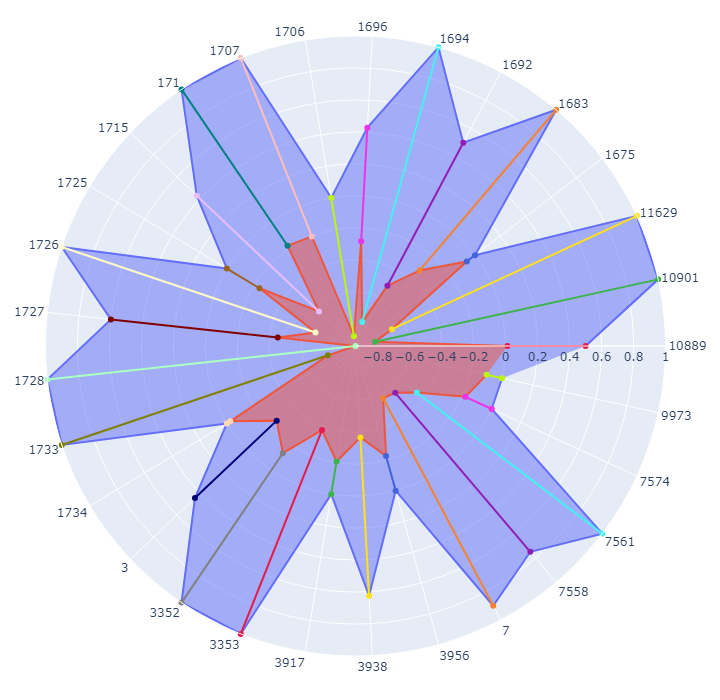
\includegraphics[width=0.7\textwidth]{images/echo_chambers_santo_andre_social_pressure.png}
	\caption{Pressão Social nas Comunidades identificadas como câmara de eco em Santo André}
	\label{fig:echo_chambers_santo_andre_social_pressure}
\end{figure}

A Comunidade 233, a qual manifesta uma inclinação para a persona \textit{helper}, como visto na atividade relacionada à poda de árvores, com um score de sentimento ligeiramente positivo e uma persona média bastante alta, reflete um envolvimento comunitário construtivo. A poda de árvores, embora possa parecer trivial, desempenha um papel crucial na manutenção da infraestrutura urbana e na prevenção de danos potenciais, sugerindo que os usuários dessa comunidade estão ativamente engajados em manter a ordem e estética de seu ambiente, além de prevenir problemas maiores.

A Comunidade 225, por outro lado, apresenta um cenário mais crítico. Com eventos tais como esgoto a céu aberto e fiscalização de obras particulares recebendo scores de sentimento fortemente negativos e uma persona consistente de \textit{complainer}, revela uma comunidade profundamente insatisfeita e preocupada com questões de saúde pública e regulamentação urbana. O esgoto a céu aberto, por exemplo, não só representa um risco à saúde como também uma falha grave na infraestrutura urbana, o que ressalta a gravidade com que tais questões são vistas pelos cidadãos.

A Comunidade 160, emerge um mosaico mais complexo de reações cívicas. Aqui, encontramos desde a preocupação com a falta de sinalização e infraestrutura básica, como exemplificado pela placa de sinalização quebrada/inexistente, até questões ambientais e de saúde pública como focos de mosquito da dengue/zika. A persona média varia significativamente, com alguns eventos indicando uma postura mais de \textit{helper} e outros de \textit{complainer}. Interessantemente, eventos como mato alto apresentam um score de sentimento positivo e uma persona média que sugere uma tendência a \textit{helper}, indicando que os usuários veem tais eventos como oportunidades de melhoria, ao invés de apenas problemas a serem denunciados. Em contraste, eventos como área com risco de deslizamento, que recebe um dos scores de sentimento mais negativos e uma persona \textit{complainer}, ressaltam uma sensação de urgência e um apelo por ação imediata, embora pareça que a comunidade não se sente capaz de contribuir de maneira significativa para sua resolução, por exemplo, muitas postagens referenciam órgãos públicos e autoridades.

A Comunidade 207 também demonstra uma preocupação com a ordem social e saúde pública, como visto na reação a eventos como comércio aberto irregularmente durante a pandemia e aglomeração de pessoas, ambos com scores de sentimento negativos e uma persona unânime de \textit{complainer}. Tais dados sugerem uma vigilância ativa e uma disposição para denunciar comportamentos considerados irresponsáveis ou perigosos durante um período de crise de saúde pública.

\begin{figure}[htb]
	\centering
	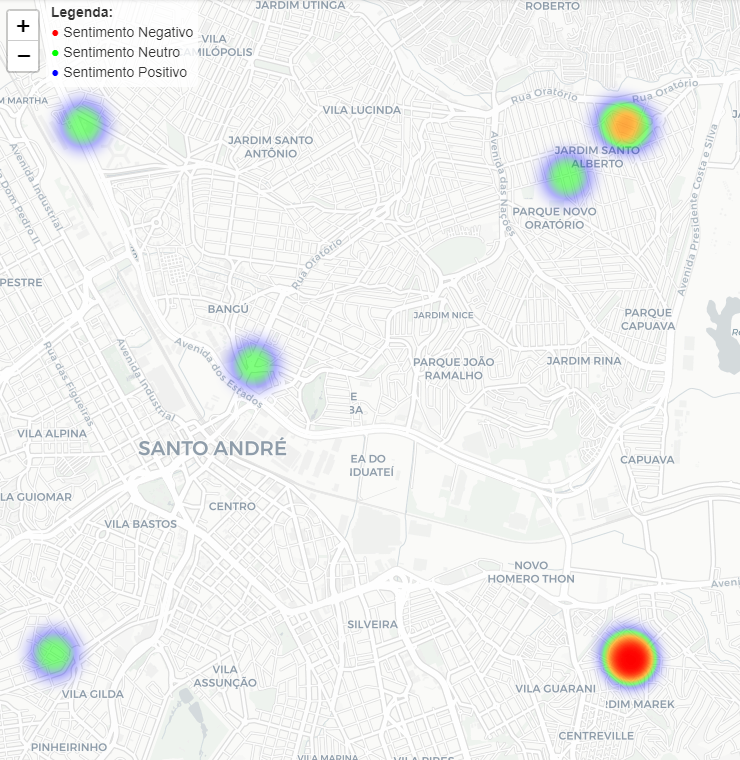
\includegraphics[width=0.7\textwidth]{images/echo_chamber_santo_andre_heatmap.PNG}
	\caption{Heatmap de Pressão Social nas Comunidades identificadas como câmara de eco em Santo André}
	\label{fig:echo_chamber_santo_andre_heatmap}
\end{figure}

Estes insights revelam que, enquanto alguns tópicos suscitam uma abordagem colaborativa e proativa por parte dos usuários, outros provocam uma resposta crítica e demandam por mudanças mais estruturais, as quais podem estar além do escopo de ação direta dos cidadãos. A presença de personas predominantemente de \textit{complainer} em eventos que refletem falhas graves de infraestrutura ou riscos à saúde pública aponta para uma comunidade que não apenas reconhece estes problemas, mas também os vê como inaceitáveis e passíveis de crítica aberta.

\subsubsection*{Visualizando Câmaras de Eco em Santo André}

\begin{figure}[htb]
	\centering
	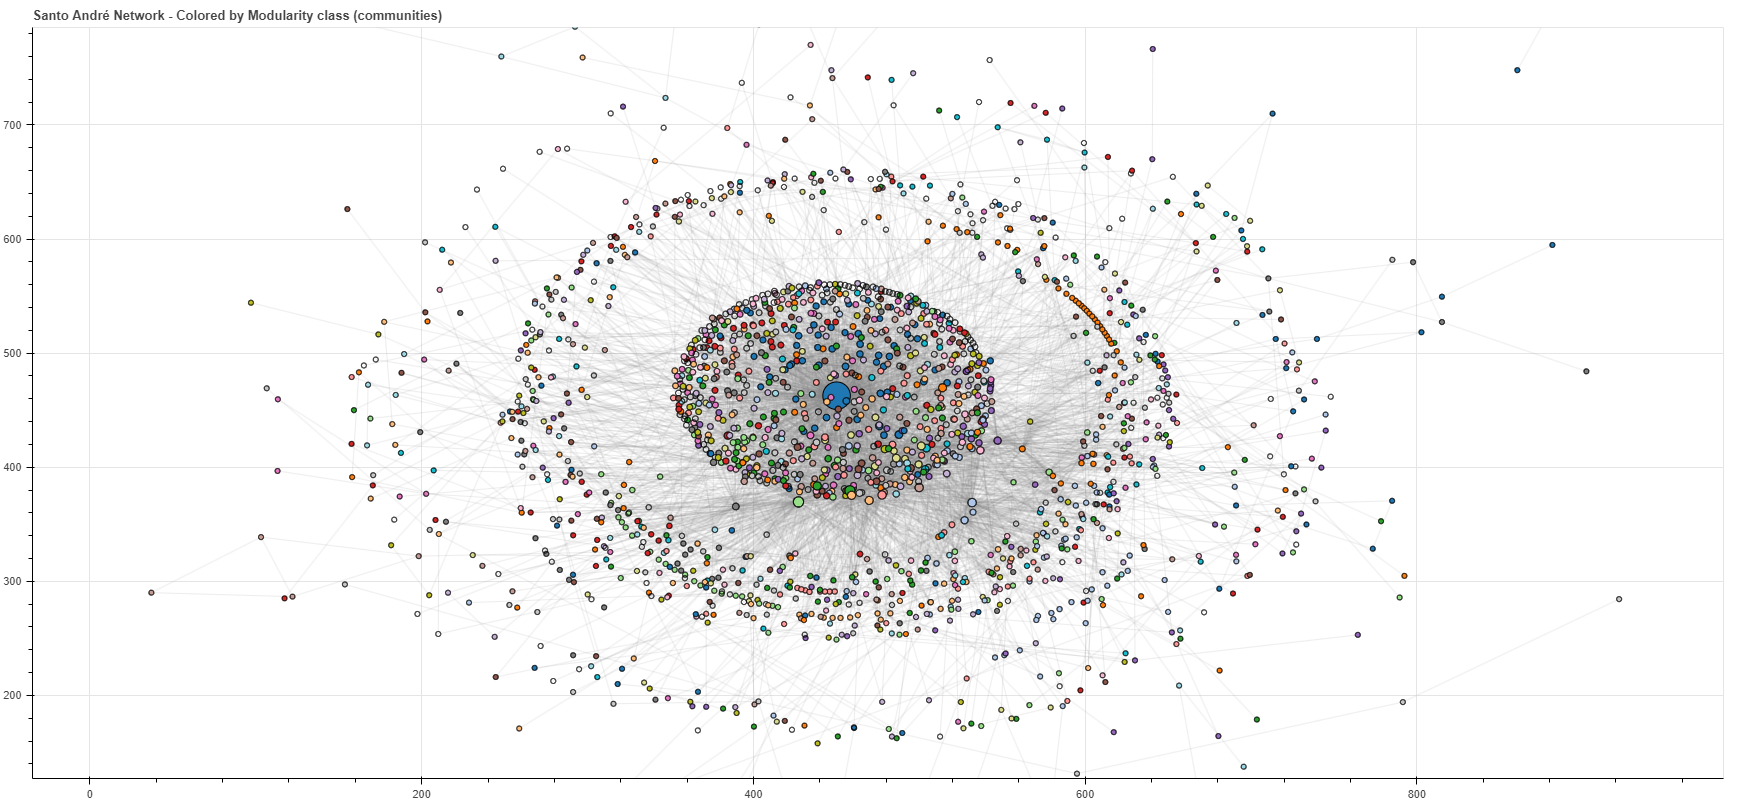
\includegraphics[width=0.95\textwidth]{images/network_community_santo_andre.png}
	\caption{Visualização das Comunidades da Rede de Santo André}
	\label{fig:network_community_santo_andre}
\end{figure}

\begin{figure}[htb]
	\centering
	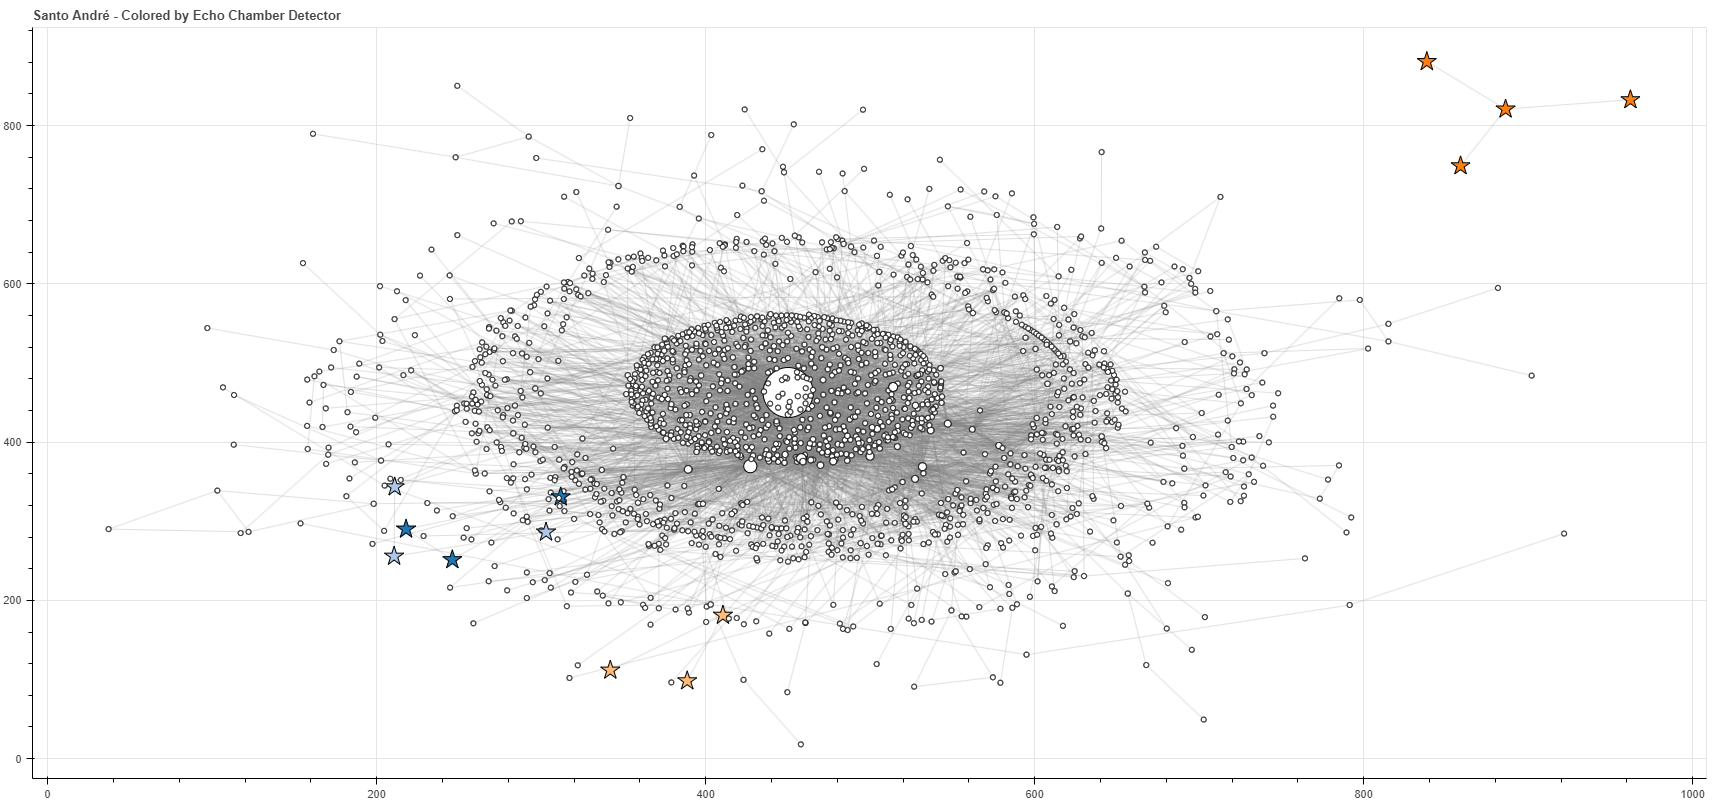
\includegraphics[width=0.95\textwidth]{images/echo_chambers_santo_andre.png}
	\caption{Visualização das Câmaras de Eco da Rede de Santo André}
	\label{fig:echo_chambers_santo_andre}
\end{figure}

Ao analisar o gráfico das câmaras de eco na rede social da cidade de Santo André, observa-se uma estrutura complexa onde certos nós agem como pontos centrais de convergência e disseminação de informações. O nó identificado como hub principal, com a maior centralidade de grau, sugere ser um influenciador chave dentro da rede, com potencial para afetar ou ser afetado por uma gama diversa de interações sociais. Notavelmente, a comunidade 233 revela-se não apenas proximamente vinculada a este hub central, mas também possivelmente atuante como um ponto de transição entre o hub e outras câmaras de eco, possivelmente funcionando como um intermediário de ideias e influências.

Contrastando com a posição centralizada da comunidade 233, identificamos que os nós da comunidade 225 estão mais periféricas na rede. Esta localização pode indicar que tais comunidades desenvolvem diálogos internos com menor interferência externa, o que pode levar a uma consolidação mais forte de perspectivas compartilhadas, reforçando o fenômeno de câmaras de eco. A formação de cliques, grupos altamente conectados dentro das câmaras de eco, é particularmente notável, pois reflete uma tendência de comunicação insular que pode exacerbar a homogeneidade de opiniões e diminuir a exposição a perspectivas divergentes.

Estes cliques, representados por conjuntos dessas duas comunidades, ilustram microcosmos onde o reforço mútuo de crenças e opiniões é provável. A presença desses cliques dentro das câmaras de eco destaca a potencial intensificação da polarização ideológica, uma vez que os membros desses grupos estão predispostos a interagir majoritariamente entre si, potencializando a circulação de um conjunto restrito de informações e pontos de vista.

A compreensão dessas dinâmicas é crucial para o desenvolvimento de estratégias de comunicação e intervenção que visem promover a diversidade de pensamento e o diálogo entre diferentes grupos sociais. As autoridades locais e organizações da sociedade civil poderiam utilizar essa análise para identificar pontos de intervenção, com o objetivo de fomentar uma maior integração comunitária e mitigar a formação de câmaras de eco que possam contribuir para a divisão social em Santo André. Esta análise aprofundada leva em conta não apenas a proximidade espacial dos nós em relação ao hub principal, mas também a qualidade das conexões e o potencial impacto dessas estruturas na comunicação e na formação de opinião dentro da rede.

\subsection{Mesquita}

\begin{table}[ht]
	\centering
	\caption{Métricas de Detecção de Câmaras de Eco da Rede da Cidade de Mesquita}
	\label{tab:echo-chamber-metrics-mesquita}
	\begin{tabular}{l|l}
		\toprule
		\textbf{Topologia da Rede}          & \textbf{Valor}                   \\
		\midrule
		Nós                                 & 933                              \\
		Arestas                             & 3578                             \\
		Nº de comunidades                   & 79                               \\
		\toprule
		\textbf{Conteúdo}                   & \textbf{Valor}                   \\
		\midrule
		Tamanho da maior comunidade         & 32                               \\
		Tamanho da menor comunidade         & 3                                \\
		Tamanho médio das comunidades       & 5.78                             \\
		Nº de comentários                   & 40924                            \\
		Nº de likes                         & 156865                           \\
		Nº de votos                         & 10355                            \\
		\midrule
		\textbf{Parâmetro Beta}             & \textbf{Valor}                   \\
		\midrule
		Beta 1                              & 0.3088                           \\
		Beta 2                              & 0.0476                           \\
		Beta 3                              & 0.5                              \\
		Beta 4                              & 0.0157                           \\
		Beta 5                              & 1                                \\
		Beta 6                              & 0.4906                           \\
		Beta 7                              & 0.0011                           \\
		\midrule
		\textbf{Polarização e Homofilia}    &                                  \\
		\midrule
		Coeficiente Global de Câmara de Eco & 0.03213                          \\
		Força da Câmara de Eco no Grafo     & 1.0982                           \\
		Nº de Câmaras de Eco Detectadas     & 8                                \\
		\midrule
		\textbf{Comunidade}                 & \textbf{Índice de Câmara de Eco} \\
		\midrule
		Comunidade 65                       & 2.3062                           \\
		Comunidade 52                       & 2.1801                           \\
		Comunidade 53                       & 2.0651                           \\
		Comunidade 54                       & 2.0548                           \\
		Comunidade 71                       & 1.9880                           \\
		Comunidade 66                       & 1.9604                           \\
		Comunidade 75                       & 1.9221                           \\
		Comunidade 61                       & 1.9030                           \\
		\bottomrule
	\end{tabular}
\end{table}

A análise realizada da rede de Mesquita destaca uma dinâmica complexa de interações sociais e a presença de potenciais câmaras de eco. Com um total de 933 nós e 3.578 arestas, a rede apresenta uma estrutura bastante interconectada. Ao analisar as comunidades dentro da rede, identificou-se um total de 79 comunidades, variando em tamanho de 3 a 32 membros, com uma média de tamanho de comunidade de aproximadamente 5.78. Isto indica uma diversidade de grupos de discussão e interação na plataforma.

Os valores de Modularidade, Coeficiente Global de Câmara de Eco (GEC) e a Força da Câmara de Eco no Grafo são indicadores cruciais da estrutura da rede e da presença de câmaras de eco. A modularidade sugere uma estrutura comunitária bem definida. O GEC indica a tendência global da rede em formar câmaras de eco, enquanto Força da Câmara de Eco de 1.0982 reflete a força das câmaras de eco dentro da rede.

\subsubsection*{Comunidades identificadas como potenciais câmaras de eco}

\begin{table}[ht]
	\centering
	\caption{Resumo das Métricas de câmaras de eco das Comunidades}
	\label{tab:community-metrics-mesquita}
	\resizebox{\textwidth}{!}{%
		\begin{tabular}{l|cccccc}
			\toprule
			\textbf{Comunidade} & \textbf{Fator de Câmara de Eco} & \textbf{Densidade} & \textbf{Homogeneidade} & \textbf{Conexões Externas} & \textbf{ECC} & \textbf{Exposição Média} \\
			\midrule
			65                  & 2.305                           & 1                  & 0.3782                 & 0.4545                     & 0.3782       & 0.5152                   \\
			52                  & 2.0757                          & 0.8333             & 0.7117                 & 0.375                      & 0.7117       & 0.4444                   \\
			53                  & 1.9353                          & 0.8333             & 0.5619                 & 0.1667                     & 0.5619       & 0.5333                   \\
			54                  & 2.1601                          & 0.5                & 0.5242                 & 0.5714                     & 0.5242       & 0.5595                   \\
			71                  & 2.1159                          & 0.3333             & 0.375                  & 0.6667                     & 0.375        & 0.5444                   \\
			66                  & 2.0464                          & 0.6667             & 0.3291                 & 0.4286                     & 0.3291       & 0.5152                   \\
			75                  & 1.7704                          & 0.3333             & 0.312                  & 0.5                        & 0.312        & 0.359                    \\
			61                  & 1.9738                          & 0.3333             & 0.267                  & 0.6667                     & 0.267        & 0.4167                   \\
			\bottomrule
		\end{tabular}
	}
\end{table}

Das 79 comunidades identificadas, 8 foram destacadas como potenciais câmaras de eco, com valores do Índice de Câmara de Eco variando de 1.903 a 2.306. Isto sugere que, enquanto a maioria das comunidades na rede apresenta uma diversidade de opiniões, estas 8 comunidades mostram uma homogeneidade notável nas opiniões e interações mais limitadas a membros da própria rede.

Ao analisar mais detalhadamente essas comunidades, observamos várias tendências:

\begin{itemize}
	\item Comunidade 65: Essa comunidade tem uma densidade 1, indicando uma interconexão completa entre seus membros. No entanto, a homogeneidade de 0.3782 e uma média de exposição de 0.5152 mostram que há um grau significativo de concordância dentro da comunidade e uma tendência para os membros serem expostos a opiniões semelhantes.
	\item Comunidade 52: apresenta uma densidade mais baixa de 0.8333, mas uma alta homogeneidade de 0.7117, refletindo uma forte concordância nas opiniões. Além disso, a baixa taxa de conexões externas indica que os membros desta comunidade têm interações limitadas fora dela, potencialmente restringindo a diversidade de informações.
	\item Comunidade 71: Com uma densidade mais baixa de 0.3333 e conexões externas de 0.6667, mostram uma interação mais diversificada, mas ainda assim apresentam características de câmara de eco devido à sua homogeneidade e média de exposição.
\end{itemize}

\subsubsection*{Visualizando Câmaras de Eco em Mesquita}

Ao analisar o plot das câmaras de eco na rede da cidade de Mesquita, observa-se uma teia de interações que ressalta a complexidade do tecido social digital. Dentro deste contexto, identificam-se comunidades distintas que, através de laços de comunicação frequentes e reforçados, podem funcionar como potenciais câmaras de eco. Estas estruturas sociais são fundamentais para entender como informações e ideologias circulam e se fortalecem dentro de grupos específicos.

\begin{figure}[htb]
	\centering
	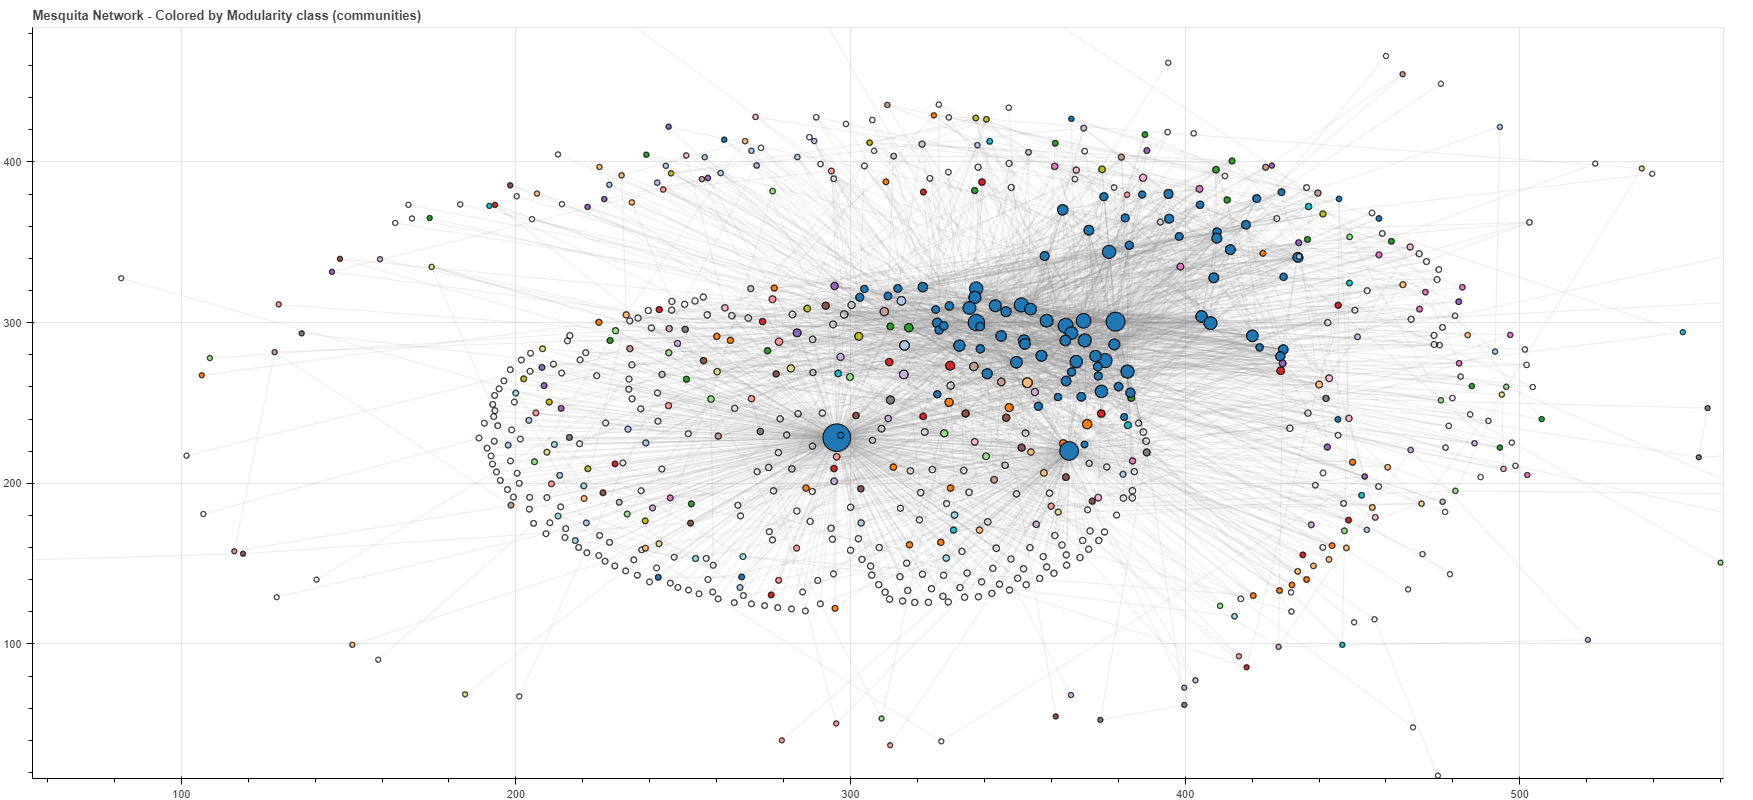
\includegraphics[width=0.95\textwidth]{images/network_communities_mesquita.png}
	\caption{Visualização das Comunidades da Rede de Mesquita}
	\label{fig:network_communities_mesquita}
\end{figure}

Neste cenário, verifica-se que alguns membros da comunidade da câmara de eco estão situados em posições estratégicas, a apenas um passo de distância do hub principal da rede. Este fato é de suma importância, pois indica não apenas uma proximidade física no espaço da rede, mas também um potencial para influência direta e troca de informações. Estes indivíduos, possivelmente atores chave na disseminação de conteúdo, ocupam posições de gatekeepers ou pontes, filtrando e direcionando o fluxo de informações.

\begin{figure}[htb]
	\centering
	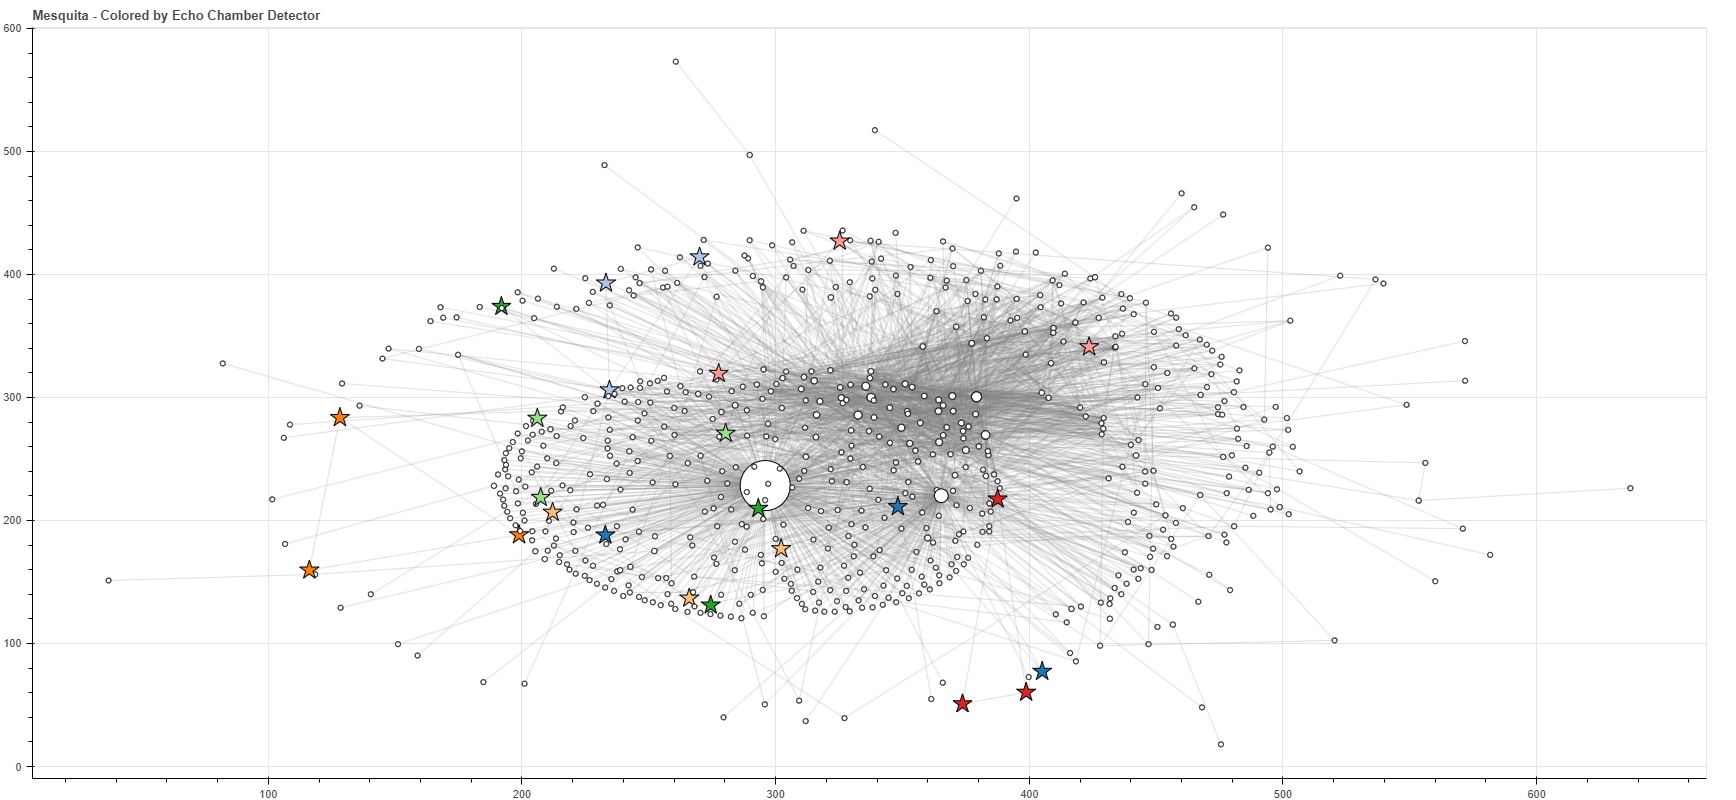
\includegraphics[width=0.95\textwidth]{images/echo_chambers_mesquita.png}
	\caption{Visualização das Câmaras de Eco da Rede de Mesquita}
	\label{fig:echo_chambers_mesquita}
\end{figure}

Além disso, a identificação de cliques inteiramente compostos por membros da comunidade da câmara de eco ilumina a presença de subgrupos altamente coesos. Tais subgrupos são caracterizados por uma forte tendência à uniformidade de opinião e podem exacerbar o fenômeno de polarização. O diálogo dentro desses cliques tende a reforçar crenças pré-existentes, minimizando a exposição a perspectivas alternativas e potencialmente criando um solo fértil para a disseminação de desinformação.

A presença dessas estruturas fechadas e auto-referenciais é particularmente relevante em contextos onde a informação é um vetor de poder e influência. Dentro das câmaras de eco, o intercâmbio de ideias tende a seguir um padrão homogêneo, onde a informação é reciclada e reverberada, amplificando crenças e opiniões com pouca ou nenhuma contestação. Este processo pode levar a uma distorção da realidade percebida, afetando a tomada de decisões e a formação de consensos em um nível mais amplo. A análise destas dinâmicas é crucial para o entendimento de como as comunidades digitais se formam e operam, bem como para o desenvolvimento de estratégias que promovam o diálogo construtivo e a diversidade de pensamento.

\subsection{Niterói}

\begin{table}[ht]
	\centering
	\caption{Métricas de Detecção de Câmaras de Eco da Rede da Cidade de Niterói}
	\label{tab:echo-chamber-metrics-niteroi}
	\begin{tabular}{l|l}
		\toprule
		\textbf{Topologia da Rede}          & \textbf{Valor}                   \\
		\midrule
		Nós                                 & 4274                             \\
		Arestas                             & 14175                            \\
		Nº de comunidades                   & 542                              \\
		\toprule
		\textbf{Conteúdo}                   & \textbf{Valor}                   \\
		\midrule
		Tamanho da maior comunidade         & 159                              \\
		Tamanho da menor comunidade         & 3                                \\
		Tamanho médio das comunidades       & 7.36                             \\
		Nº de comentários                   & 80731                            \\
		Nº de likes                         & 199668                           \\
		Nº de votos                         & 11640                            \\
		\midrule
		\textbf{Parâmetro Beta}             & \textbf{Valor}                   \\
		\midrule
		Beta 1                              & 0.0789                           \\
		Beta 2                              & 0.01886                          \\
		Beta 3                              & 0.11117                          \\
		Beta 4                              & 0.00144                          \\
		Beta 5                              & 1                                \\
		Beta 6                              & 0.51574                          \\
		Beta 7                              & 0.00023                          \\
		\midrule
		\textbf{Polarização e Homofilia}    &                                  \\
		\midrule
		Coeficiente Global de Câmara de Eco & 0.0213                           \\
		Força da Câmara de Eco no Grafo     & 1.05116                          \\
		Nº de Câmaras de Eco Detectadas     & 1                                \\
		\midrule
		\textbf{Comunidade}                 & \textbf{Índice de Câmara de Eco} \\
		\midrule
		Comunidade 515                      & 2.066647                         \\
		\bottomrule
	\end{tabular}
\end{table}

Ao analisar as métricas de detecção de câmaras de eco geradas para a rede da cidade de Niterói, encontramos diversos pontos de interesse que lançam luz sobre a dinâmica da rede e a possibilidade de câmaras de eco em seu interior. A topologia da rede é notável com um grande volume de nós e arestas, indicando uma rede social relativamente densa. No entanto, a divisão em 542 comunidades revela uma fragmentação significativa, com uma média de apenas cerca de 7.36 membros por comunidade. A maior comunidade contém 159 membros, enquanto a menor tem apenas 3. A análise da modularidade revela uma estrutura razoavelmente dividida em subgrupos, com um valor de 0.515. Quando examinamos o conteúdo da rede, observamos um grande volume de atividade, com 80731 comentários, 199668 likes e 11640 votos. Esses números indicam uma rede social ativa e engajada, onde os usuários interagem regularmente.

A análise dos parâmetros Beta oferece insights adicionais. Os valores desses parâmetros variam, sugerindo que diferentes aspectos da rede podem influenciar a formação de câmaras de eco. Por exemplo, Beta 3, com um valor de 0.11117, indica que a presença de conexões externas pode ser um fator importante na prevenção da formação de câmaras de eco, enquanto Beta 6, com um valor de 0.51574, sugere que o coeficiente de câmara de eco global (GEC) desempenha um papel significativo.

No que diz respeito à polarização e homofilia, o coeficiente global de câmara de eco (GEC) é relativamente baixo, com um valor de 0.0213. Isso pode indicar que a rede como um todo não está fortemente polarizada, o que é uma boa notícia em termos de diversidade de perspectivas. No entanto, a força da câmara de eco no grafo, com um valor de 0.95116, sugere que, quando as câmaras de eco estão presentes, elas têm uma influência significativa.

A detecção identificou apenas uma comunidade como uma potencial câmara de eco, com um índice de câmara de eco de 2.066647. Isso é intrigante, pois sugere que, embora a rede como um todo não seja fortemente polarizada, existe pelo menos uma comunidade que demonstra uma notável homogeneidade em suas opiniões e perspectivas. A existência de apenas uma comunidade identificada como potencial câmara de eco pode ser atribuída a vários fatores.

Primeiro, pode ser devido à forma como as comunidades são definidas ou particionadas na rede. Se a detecção de comunidades não for sensível o suficiente para identificar subdivisões dentro das comunidades maiores, isso poderia resultar na identificação de apenas uma câmara de eco.

Segundo, as características específicas da rede de Niterói podem influenciar esse resultado. Por exemplo, a natureza das interações entre os membros da comunidade, a distribuição de opiniões e a presença de influenciadores podem variar amplamente de uma rede para outra. Essas peculiaridades podem fazer com que algumas redes sejam mais propensas a formar câmaras de eco do que outras.

Por fim, é importante mencionar que o ajuste de parâmetros nas heurísticas de partição de comunidades também pode afetar os resultados. Experimentos anteriores indicam que mesmo pequenas alterações nos parâmetros podem levar a diferentes resultados na detecção de câmaras de eco. No entanto, ao repetir a detecção utilizando outras heurísticas de partição de comunidades e parâmetros beta, observamos que a presença de certos usuários na comunidade 515 pode influenciar negativamente a dinâmica da comunidade, aumentando a probabilidade de polarização ao longo do tempo. Em outras palavras, a centralidade e as características desses usuários tendem a direcionar a comunidade em direção à formação de uma câmara de eco, dependendo da sua influência na comunidade.

Em resumo, a análise das métricas de detecção de câmaras de eco para a rede da cidade de Niterói revela uma rede social ativa e fragmentada, com uma comunidade identificada como potencial câmara de eco. Embora a rede como um todo não pareça fortemente polarizada, essa descoberta destaca a importância de compreender as nuances da dinâmica da rede e as características específicas que podem influenciar a formação de câmaras de eco em contextos sociais.

\subsubsection*{Comunidade 515}

\begin{table}[ht]
	\centering
	\caption{Métricas de Detecção de Câmaras de Eco da Comunidade 515 de Niterói}
	\label{tab:echo-chamber-metrics-community515}
	\begin{tabular}{l|l}
		\toprule
		\textbf{Métrica}                   & \textbf{Valor} \\
		\midrule
		Fator de Câmara de Eco             & 1.8582         \\
		Densidade                          & 0.3333         \\
		Homogeneidade                      & 0.271          \\
		Conexões Externas                  & 0.6            \\
		ECC (Coeficiente de Câmara de Eco) & 0.571          \\
		GEC (Coeficiente Global de Eco)    & 0.0321         \\
		Exposição Média                    & 0.3704         \\
		\bottomrule
	\end{tabular}
\end{table}

Essas particularidades nos convidam a examinar as métricas de detecção de câmaras de eco da Comunidade 515 de Niterói, conforme apresentadas na Tabela \ref{tab:echo-chamber-metrics-community515}. Essas métricas oferecem insights valiosos sobre a dinâmica e o potencial de formação de câmaras de eco dentro desta comunidade específica.

Ao observar o Fator de Câmara de Eco, que apresenta um valor de 1.8582, podemos inferir que essa comunidade possui uma tendência significativa a formar câmaras de eco. Este valor, que é maior que 1, indica que os membros desta comunidade têm uma exposição predominantemente alta a informações que reforçam suas crenças e opiniões preexistentes. Isso sugere que os indivíduos na Comunidade 515 estão mais propensos a interagir com conteúdo e opiniões que estão alinhados com suas próprias visões, o que pode contribuir para uma polarização de opiniões dentro da comunidade.

A densidade, com um valor de 0.3333, significa que os membros desta comunidade estão moderadamente interconectados. Embora não seja uma densidade extremamente alta, essa interconexão ainda indica que os membros têm uma rede de comunicação relativamente sólida dentro da comunidade, o que pode facilitar a formação de câmaras de eco. A homogeneidade das opiniões, representada por um valor de 0.571, também é relevante. Esse número sugere que existe uma concordância ou semelhança mediana nas opiniões dos membros da Comunidade 515. Portanto, essa métrica indica que as opiniões compartilhadas dentro desta comunidade têm uma certa uniformidade, o que é um fator que contribui para a formação de câmaras de eco. As "Conexões Externas" da comunidade, avaliada em 0.6, mostra que os membros da têm uma quantidade considerável de interações com indivíduos ou grupos fora da comunidade. Essas conexões externas podem atenuar, em certa medida, a formação de câmaras de eco, já que a exposição a perspectivas divergentes é mais provável quando há conexões externas significativas.

O "ECC" (Coeficiente de Câmara de Eco) tem um valor de 0.271, que está em concordância com a homogeneidade das opiniões. Isso significa que a probabilidade de um membro desta comunidade se isolar em uma câmara de eco é relativamente alta. Por outro lado, o "GEC" (Coeficiente Global de Eco) apresenta um valor de 0.0321. Esse valor mais baixo indica que, considerando a rede como um todo, a tendência à formação de câmaras de eco não é tão proeminente. No entanto, as métricas individuais dentro da Comunidade 515 revelam que essa comunidade específica tem uma dinâmica interna que favorece a formação de câmaras de eco. Por fim, a "Exposição Média" na comunidade, com um valor de 0.3704, indica que, em média, os membros são frequentemente expostos a opiniões e conteúdo que estão alinhados com suas próprias visões, contribuindo para o fenômeno da câmara de eco.

Ao análisar a comunidade 515 de Niterói com as heurísticas de pressão social descritas no capítulo anterior, algumas particularidades interessantes são reveladas, que podem ajudar a entender por que essa foi a única câmara de eco identificada. A comunidade consiste em um grupo relativamente pequeno, com apenas 8 membros. Essa pequena dimensão pode contribuir para a formação de uma câmara de eco, pois a interação limitada com perspectivas externas pode levar a uma maior homogeneidade de opiniões.

\begin{figure}[htb]
	\centering
	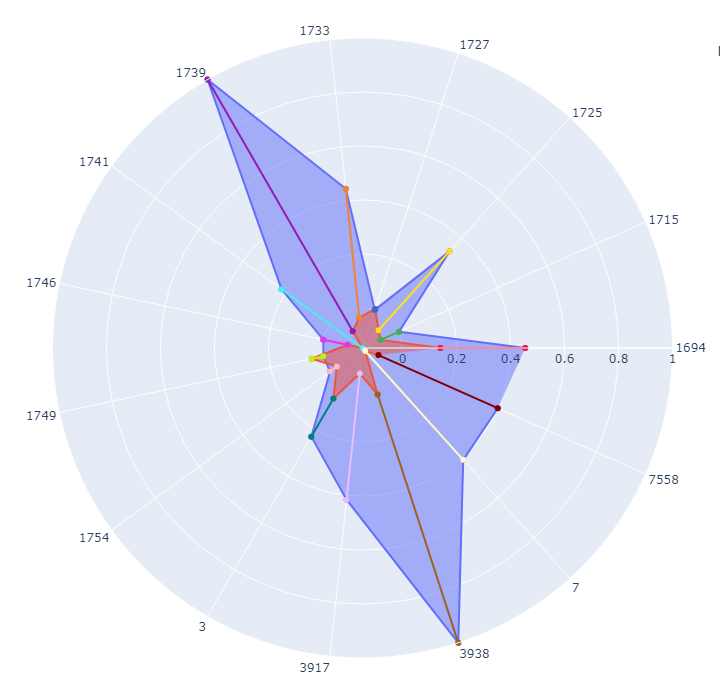
\includegraphics[width=0.7\textwidth]{images/niteroi_community_515.png}
	\caption{Gráfico de radar ilustrando as métricas de pressão social da Comunidade 515 de Niterói}
	\label{fig:niteroi_community_515}
\end{figure}

Considerando aspectos de conteúdo e criação de eventos no Colab, os membros da comunidade criaram um total de 180 eventos, o quedemonstra um alto nível de engajamento e atividade dentro da comunidade. Além disso, os membros da comunidade deram um total de 9.975 likes. Esse número é notavelmente alto em relação ao número de usuários na comunidade, sugerindo que eles têm uma tendência a apoiar e endossar as opiniões e eventos na rede. Foram realizados 256 votos up/down em eventos de outros usuários. A comunidade fez 1.202 comentários em eventos de outros usuários. Esses indicadores de engajamento mostram que os membros da comunidade estão ativamente envolvidos na rede e estão dispostos a se envolver em discussões com membros externos à comunidade.

Os tipos de eventos mais comuns na comunidade 515 estão relacionados a problemas e reclamações em infraestrutura urbana, como lâmpadas apagadas à noite, pontos de infração de trânsito recorrentes, buracos nas vias e calçadas irregulares. Esses eventos podem gerar discussões e interações específicas dentro da comunidade, contribuindo para a formação de uma câmara de eco em torno desses tópicos. A análise da persona dos usuários mostra que a maioria deles tende a ser \textit{complainer}. Isso indica uma predisposição para expressar opiniões negativas e reclamações, o que pode amplificar a polarização e a formação de câmaras de eco. A análise do sentimento das postagens revela que a maioria dos eventos tem um sentimento negativo, polarizando ainda mais as opiniões dentro da comunidade.

Embora haja um número significativo de eventos criados, eles estão concentrados em alguns tópicos específicos, como problemas de infraestrutura urbana e trânsito. A falta de diversidade de tópicos pode contribuir para a formação de uma câmara de eco, pois os membros da comunidade estão focados em um conjunto limitado de preocupações. Ao analisar os eventos criados pelos membros das comunidades, observamos que um tópico recorrente de discussão parece envolver as dinâmicas de trânsito e estacionamento no centro da cidade. Os usuários demonstram com scores majoritariamente negativos, descontentamento sobre a falta de vagas de estacionamento bem como multas que receberam e consideram injustas, principalmente porque muitas das postagens também denunciam infranções cometidas por outros motoristas e parecem cobrar uma multa do poder público. Além disso, os usuários parecem reclamar da falta de sinalização e de fiscalização por parte da prefeitura, evidenciado pelos eventos criados no tópico Manutenção/implantação de placa de sinalização, com 10 eventos criados.

\begin{figure}[htb]
	\centering
	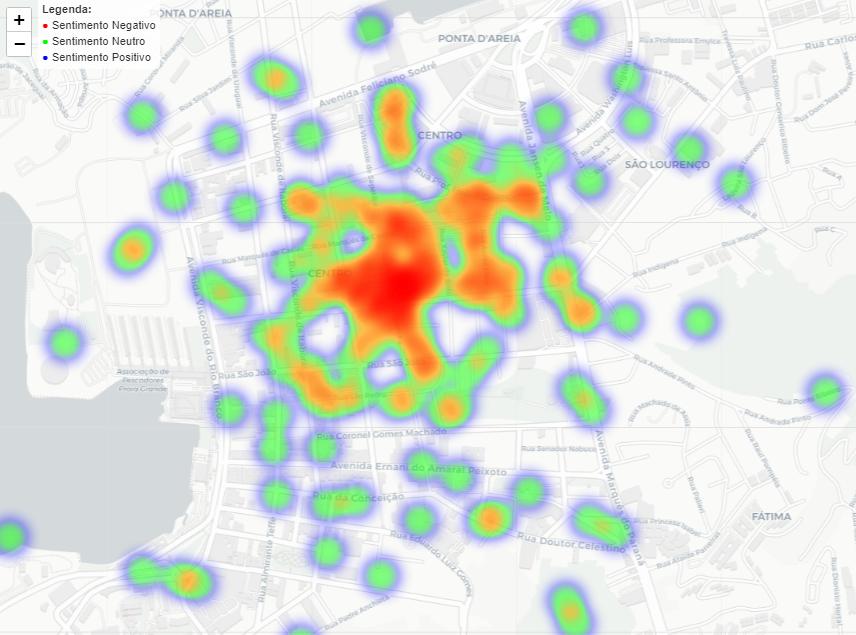
\includegraphics[width=0.7\textwidth]{images/echo_chamber_niteroi_heatmap.PNG}
	\caption{Heatmap ilustrando a distribuição de tópicos na comunidade 515 no mapa de Niterói}
	\label{fig:echo_chamber_niteroi_heatmap}
\end{figure}

A comunidade 515 de Niterói se destaca por sua intensa atividade relacionada a problemas e reclamações na infraestrutura urbana, abordando questões como iluminação noturna deficiente, pontos de infração de trânsito recorrentes e condições precárias de vias e calçadas. Essa concentração em tópicos específicos pode ser um fator-chave na identificação dessa comunidade como uma câmara de eco. Além disso, a análise da persona dos usuários revela uma tendência significativa para expressar opiniões negativas e reclamações, o que contribui para a amplificação da polarização. A predominância de postagens com sentimentos negativos dentro da comunidade também intensifica essa polarização. Esses fatores, combinados, contribuem para a identificação da comunidade 515 como uma câmara de eco, onde opiniões similares são amplificadas, resultando em uma polarização acentuada em torno desses problemas específicos.

\subsubsection*{Visualizando Câmaras de Eco em Niterói}

\begin{figure}[htb]
	\centering
	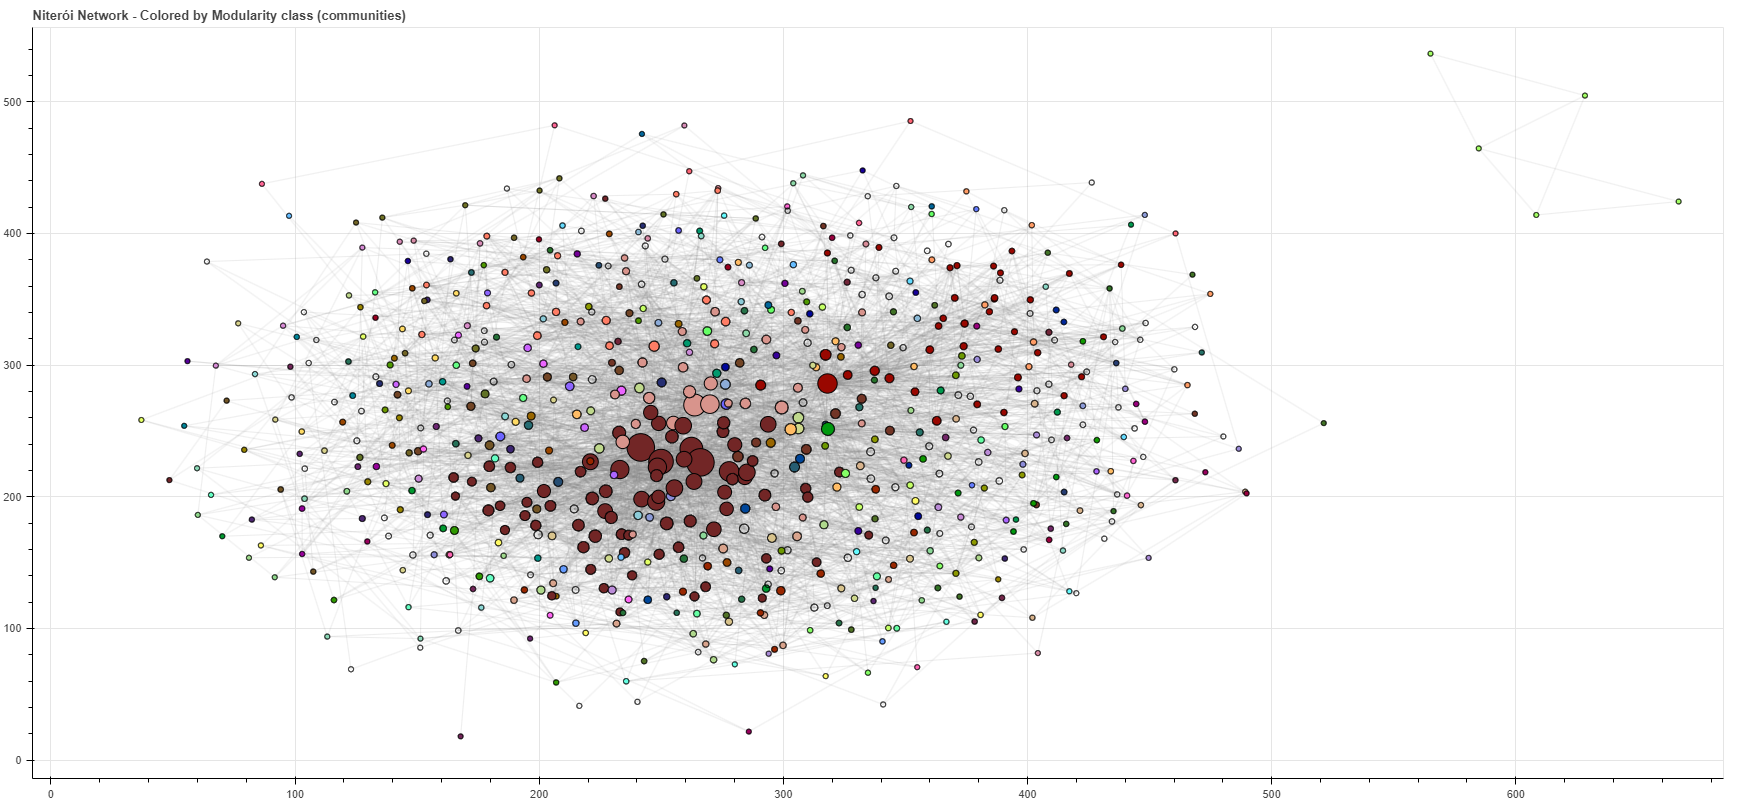
\includegraphics[width=0.95\textwidth]{images/network_communities_niteroi.png}
	\caption{Visualização das Comunidades da Rede de Niterói}
	\label{fig:network_communities_niteroi}
\end{figure}

Ao analisar o gráfico das câmaras de eco na rede social da cidade de Niterói, percebe-se que a centralidade de conexões é dominada pelo hub principal, identificado pelo nó 113450. Este nó se destaca como uma entidade significativa dentro da rede, provavelmente desempenhando um papel crucial na difusão de informações. A comunidade indicada como alta probabilidade de ser câmara de eco, não apresentou membros notoriamente próximos desse hub central. No entanto, a existência de cliques fortes na comunidade, onde todos os usuários seguem e são seguidos pelos outros usuários, evidencia a presença de comunicações intensas e circuitos fechados de informação entre esses indivíduos. A comunidade, que possui 5 usuários, tem 2 cliques, de 3 e 2 usuários respectivamente, além de serem interconectados por um usuário que faz parte dos dois cliques. Estes subgrupos altamente interconectados são característicos de câmaras de eco, onde o isolamento de membros de influências externas pode levar a uma polarização e a uma visão de mundo uniformizada. O entendimento dessas microestruturas é fundamental para decifrar as dinâmicas de informação e influência na cidade, oferecendo pistas sobre como ideias e crenças podem ser fortalecidas dentro de comunidades fechadas e como intervenções podem ser desenhadas para promover um discurso mais aberto e diversificado.

\begin{figure}[htb]
	\centering
	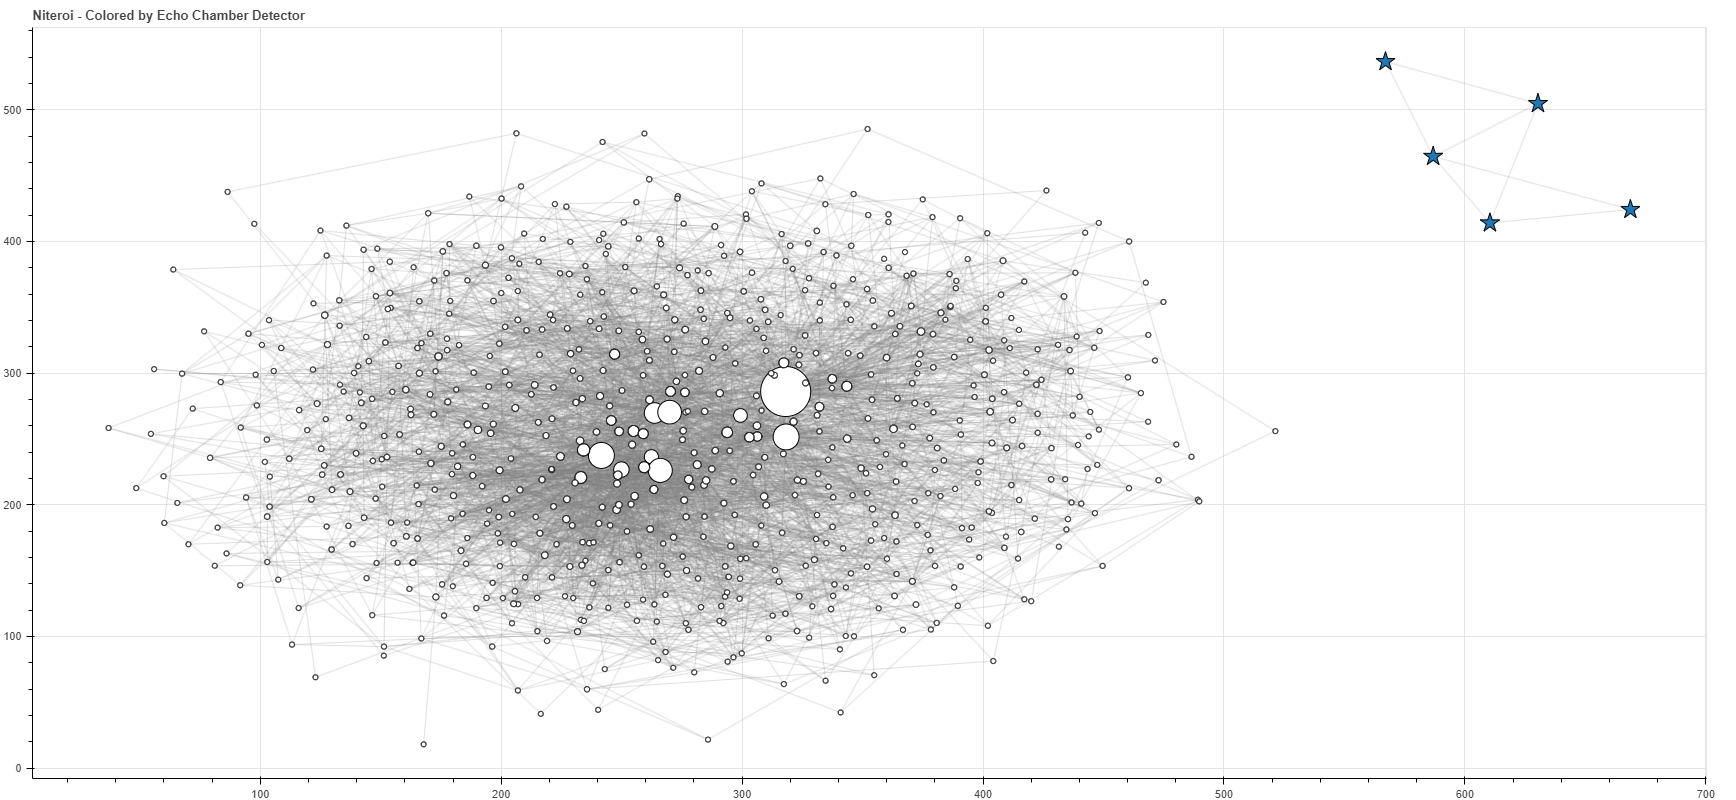
\includegraphics[width=0.95\textwidth]{images/echo_chambers_niteroi.png}
	\caption{Visualização das Câmaras de Eco da Rede de Niterói}
	\label{fig:echo_chambers_niteroi}
\end{figure}

Sob a perspectiva de análise de redes sociais, Niterói destaca-se como um espaço digital intrigante onde a densidade e modularidade moderada coexistem com sentimentos negativos e polarizados, especialmente em temas de mobilidade urbana, gerando uma alta pressão social sobre este tópico. Apesar desta polarização, a cidade demonstrou um engajamento diversificado em diferentes tópicos de pressão social e uma alta porcentagem de usuários com persona \textit{helper}, contribunindo para a heteogngnei de opiniões e a interações com outras perspectivas, melhorando a exposição média dos usuários, o que ajuda a equilibrar a polaridade da rede como um todo. No entanto, uma métrica GEC superior a 1 apontou a possibilidade de câmaras de eco na rede, ou que comunidades mais polarizadas possam estar em um processo de formação de câmara de eco. Dentre estas, a heurística de detecção de câmaras de eco identificou a Comunidade 515 como o único ambiente com parâmetros suficientes para ser considerado um espaço de alta polarização e homogeneidade de opiniões.

A análise detalhada da Comunidade 515 confirmou os aspectos de alta polarização e homogeneidade de opiniões, especialmente relacionadas a questões de trânsito no centro da cidade, caracterizando-a como uma câmara de eco. O plot de heatmap da pressão social exercida pela Comunidade 515 no mapa de Niterói corroborou que a maioria dos usuários desta comunidade atua em eventos de trânsito no centro, exercendo uma forte pressão social nesta localidade. Este estudo revela a importância de analisar as redes sociais em um nível granular para entender a dinâmica de comunidades específicas que podem estar em desacordo com a dinâmica geral da rede. A identificação e análise de tais comunidades polarizadas podem fornecer insights valiosos para as autoridades locais e administradores de plataformas, permitindo uma resposta mais informada e possivelmente, a criação de estratégias para promover o diálogo e a diversidade de opiniões, mitigando a formação de câmaras de eco e polarização excessiva em questões críticas de infraestrutura urbana.

\section{Discussão dos Resultados}

O fenômeno das câmaras de eco nas redes sociais emerge como um desafio central na era da informação digital, onde os diálogos e opiniões estão cada vez mais polarizados e isolados. Este capítulo buscou identificar e analisar as câmaras de eco nas redes sociais das cidades de Santo André, Niterói e Mesquita, utilizando um teorema matemático e um modelo de detecção baseado em métricas de pressão social, homogeneidade de opiniões e topologia de rede. A relevância deste estudo se ancora na necessidade de entender como as estruturas sociais digitais podem influenciar a formação de opiniões e a disseminação de informações, com potenciais implicações para o tecido social e a governança democrática.

A metodologia implementada neste estudo representa uma abordagem integrada, combinando simulação de redes sociais, análise heurística e visualização avançada. Inicialmente, empregamos o Modelo de Redes Gráficas Exponenciais (ERGM) para modelar a rede de interações sociais dos usuários do Colab. ERGM é particularmente adequado para este propósito, pois permite incorporar a estrutura e os processos sociais nas simulações de rede, refletindo as tendências e os padrões observados em dados de redes sociais reais.

Para enriquecer nossa simulação e aproximar nossos modelos da dinâmica realista do comportamento do usuário, integramos o conceito de modelagem baseada em agentes. Criamos agentes autônomos, ou "bots", programados para gerar conteúdo e interagir com outros usuários de maneira coerente com as personas identificadas na plataforma. Cada bot foi configurado com um conjunto de regras de interação e perfis de comportamento que refletem as heurísticas derivadas da análise de sentimentos e da classificação de personas, como \textit{Helpers} e \textit{Complainers}.

Essa fusão de ERGM com a modelagem baseada em agentes permite não apenas simular a estrutura da rede, mas também animar a rede com comportamentos individuais que podem influenciar a evolução da rede ao longo do tempo. A interação entre os bots é projetada para imitar as ações e reações dos usuários humanos, proporcionando insights sobre como a pressão social e a influência podem se manifestar e se espalhar através das conexões sociais. Com essa abordagem híbrida, visamos capturar a intersecção entre a topologia da rede e os processos dinâmicos que ocorrem dentro dela, oferecendo uma nova perspectiva sobre a pressão social nas redes hiperlocais do Colab.

Através das simulações, conseguimos replicar as estruturas sociais do ambiente digital com um alto grau de precisão. As heurísticas de detecção de câmaras de eco foram então aplicadas para identificar subgrupos altamente interconectados e homogêneos, potencialmente suscetíveis a efeitos de ressonância ideológica. Para complementar a análise quantitativa, técnicas de visualização foram aprimoradas, proporcionando uma representação intuitiva e acessível das estruturas da rede, destacando as potenciais comunidades em câmaras de eco.

Topologicamente, as câmaras de eco identificadas nas redes das três cidades mostraram características distintas. Santo André teve quatro comunidades identificadas, com variáveis graus de interconexão. Niterói destacou-se com uma única comunidade, que após análise do conteúdo, constatou-se através doss níveis de polaridade e baixa conexões externas como uma câmara de eco sob o tópico de pressão social  de "Infrações de Trânsito". Mesquita, por outro lado, revelou oito comunidades, com índices de câmara de eco, obtidos através de análise PCA, significativamente mais altos do que os encontrados nas outras cidades, indicando uma tendência para a homogeneidade de opiniões e a forte pressão social. 

Essas métricas de pressão social, como frequência de interações e criação de conteúdo dentro de grupos homogêneos, interagindo os mesmos tipos de evento, revelaram muito sobre os diálogos digitais das cidades. Em Mesquita, onde as métricas indicaram uma pressão social mais intensa, os diálogos tendiam a ser mais uniformes e menos diversificados, sugerindo uma rede mais suscetível à formação de câmaras de eco. Em contraste, Niterói apresentou uma variedade mais ampla de interações, o que pode ser sintomático de uma maior exposição a perspectivas diversas e um debate mais saudável.

Ao analisar a performance do modelo de detecção de câmaras de eco, principalmente ao analisar as métricas de pressão social e a polaridade das postagens criadas pelos membros da comunidade, revela uma capacidade de identificar, de maneira consistente, comunidades com alta probabilidade de serem câmaras de eco. 

Em Santo André, as quatro comunidades detectadas indicam uma rede moderadamente fragmentada, enquanto em Niterói, a presença de uma única comunidade ampla sugere uma centralização menor, porém, os tópicos dos eventos e os scores de sentimento prendominantemente negativos, sugerem que essa comundiade específica está descontente com os órgãos governamentais nas questões de trânsito no centro e as suas opiniões negativas exercem uma pressão social moderada, especialmente no centro da cidade. Em Mesquita, o alto número de comunidades com fortes indicadores de câmaras de eco sugere um ambiente digital mais isolado e polarizado. Os resultados dos experimentos forneceram evidências substanciais que corroboram nosso teorema matemático. A presença de comunidades com altos índices de câmara de eco em Mesquita, em particular, alinha-se com as previsões do teorema, destacando a influência de conexões densas e homogeneidade ideológica na formação desses subgrupos.

As comunidades identificadas como potenciais câmaras de eco oferecem insights valiosos sobre as redes das respectivas cidades. Em Santo André, a diversidade das comunidades sugere um espectro de diálogos e potenciais pontos de vista. Em Niterói, a rede centralizada pode facilitar o acesso a uma gama mais ampla de opiniões, embora isso não isente completamente o risco de polarização. Em Mesquita, a presença de múltiplas comunidades isoladas indica um ambiente propício à formação de opiniões homogêneas, reforçando a necessidade de intervenções para promover a diversidade e o diálogo.

É importante notar que devido ao tamanho das comunidades identificadas como câmaras de eco em potencial, bem como a quantidade limitada de postagens disponíveis para análise cujo o autor faz parte dessas comundiades é bem menor em comparação com algumas comunidades maiores com usuários mais antigos da rede. Essa limitação pode ter afetado a precisão das métricas de pressão social e polaridade, especialmente em Mesquita, onde a maioria das comunidades identificadas era pequena, entre 3 a 5 membros. Porém, é importante notar que, o tamanho médio das comunidades em Mesquita é de 5.78 membros, portanto a média de membro das comunidades identificadas como câmaras de eco está dentro da média de comunidades de todas as cidades, exceto Niterói. No entanto, a análise de sentimentos e a classificação de personas foram realizadas em toda a rede, o que nos permite inferir com segurança que as comunidades não identificadas como câmaras de eco não apresentam características que as tornem suscetíveis a esse fenômeno, mesmo com uma grande quantidade de dados disponíveis para essas comunidades.

Além disso, um aspecto crucial da metodologia utilizada é a capacidade de discernir câmaras de eco genuínas de comunidades com alta atividade que, de outra forma, poderiam ser equivocadamente classificadas como tal devido ao volume substancial de postagens. O algoritmo empregado demonstrou precisão, evitando falsos positivos mesmo em comunidades com numerosas postagens disponíveis para análise, o que poderia distorcer as métricas de pressão social e polaridade. Portanto, as comunidades identificadas como câmaras de eco refletem uma configuração específica de interações e não são simplesmente artefatos de um volume maior de dados.

A relação entre o modelo proposto e as técnicas de detecção de comunidades merece uma análise cuidadosa. Por exemplo, ao utilizar o algoritmo de Leiden para a identificação de comunidades, observou-se que a maior comunidade em Niterói possui 159 membros. Portanto, ao aplicar o modelo de detecção de câmaras de eco a esta comunidade, tratou-se o coletivo como uma entidade única, analisando a polaridade, homogeneidade de opiniões, conexões eternas dos 159 membros da comunidade para o grafo e as outras comunidades identificadas. Essa abordagem pode não capturar a formação de subgrupos internos. É concebível que dentro de comunidades de grande escala, subgrupos menores operem como câmaras de eco independentes. Contudo, a análise de tais subgrupos não se enquadra no escopo do presente estudo, uma vez que as heurísticas utilizadas são aplicadas ao grafo na sua totalidade e não a componentes isolados.

Essencialmente, ao considerar uma comunidade ampla como um único grafo, informações cruciais sobre conexões externas — um componente vital para a precisão do nosso modelo — podem ser obscurecidas. A análise de comunidades mais extensas como um todo, sem reconhecer a existência potencial de subgrupos, poderia levar a uma interpretação errônea das métricas de detecção de câmaras de eco. Portanto, enquanto o modelo demonstra robustez na identificação de câmaras de eco em uma escala global, ele não é otimizado para o reconhecimento de dinâmicas de câmaras de eco que possam existir dentro de subestruturas de comunidades maiores.

Os resultados deste estudo sugerem que a integração da análise de sentimentos com métricas derivadas de análise de redes sociais pode oferecer uma abordagem valiosa para a investigação da polarização. Essa combinação de metodologias fornece uma base para explorar as complexidades na dinâmica das opiniões, o que pode ser instrumental para um entendimento mais profundo da estrutura e influência das câmaras de eco.

Adicionalmente, a incorporação da classificação de personas, do score de sentimentos das postagens e dos tipos de eventos mais frequentemente engajados pelos usuários, fornece um arcabouço robusto para derivar métricas de homogeneidade de opiniões. Esta análise é aprofundada pelo fator de exposição externa a opiniões divergentes, avaliando o contraste entre os eventos que um usuário posta versus aqueles com os quais interage mais na rede. Essas métricas são particularmente pertinentes para a análise de polarização dentro de redes sociais digitais.

No contexto do Colab, uma plataforma social dedicada à cidadania, a incorporação da geolocalização das postagens adiciona uma camada significativa de insights. A combinação desses dados com o modelo de pressão social hiperlocal permite não apenas a identificação, mas também a localização de áreas com alta concentração de reclamações ou elogios, tipos específicos de eventos e o sentimento predominante relacionado a eles. Esta dimensão geográfica fornece uma perspectiva valiosa sobre onde os cidadãos estão mais vocalmente insatisfeitos ou satisfeitos, oferecendo uma ferramenta poderosa para órgãos governamentais e políticos na alocação de recursos e na resposta às preocupações dos cidadãos de maneira direcionada e eficiente.

Este estudo se posiciona na intersecção da engenharia de software e das ciências sociais, buscando trazer contribuições quantitativas para a análise de fenômenos sociais complexos, como as câmaras de eco em redes digitais. Com base em uma extensa revisão da literatura em análise de redes e a integração de métricas derivativas, assim como a adoção da modelagem baseada em agentes de Atiqi e as heurísticas de GEC e ECC, foi possível desenvolver um teorema matemático para a análise quantitativa da polaridade em comunidades online.

Através da implementação de um modelo validado com o uso de ERGM e simulações de redes que espelham as características observadas no Colab, o estudo avançou na aplicação prática de teorias matemáticas e computacionais. A incorporação de dados de análise de sentimentos e a classificação manual de postagens, refinada posteriormente por um classificador de aprendizado de máquina, forneceu os insumos essenciais para o mecanismo de detecção de câmaras de eco. Este mecanismo identificou variações significativas na constituição e dinâmica das comunidades nas três cidades estudadas — uma comunidade em Niterói, oito em Mesquita e quatro em Santo André.

A partir desses experimentos, aprendemos que as técnicas de engenharia de software podem ser aplicadas com sucesso para elucidar aspectos da dinâmica social. A análise quantitativa, apoiada por modelos matemáticos e computacionais, pipelines de pre-processamento e a classificação dos \textit{outputs} gerados oferece uma nova lente para examinar a formação e a influência das câmaras de eco. Além disso, os resultados sublinham a importância de considerar a singularidade de cada comunidade ao aplicar esses modelos, destacando como variáveis locais, como a geografia social e o comportamento dos usuários, podem afetar a manifestação de polarização e a pressão social.